\documentclass[12pt]{jsarticle}
\usepackage{fancyhdr}
\pagestyle{fancy}
\lhead{\leftmark}
\rhead{\today}

\usepackage{graphicx}

\begin{document}

\title{
  ギガマシーンダービィ \linebreak{}
  エナドリ爆発 (仮) \linebreak{}
  企画書/仕様書 (仮)
}
\author{nasuria}
\date{\today}
\maketitle
\newpage

\tableofcontents
\newpage


\section{概要}
大学生がエナドリを投げて敵を倒し、ステージを進む2Dアクション。

主人公の攻撃はチャージで形態が変わり、だんだん強化される。

\begin{figure}[htbp]
  \begin{center}
    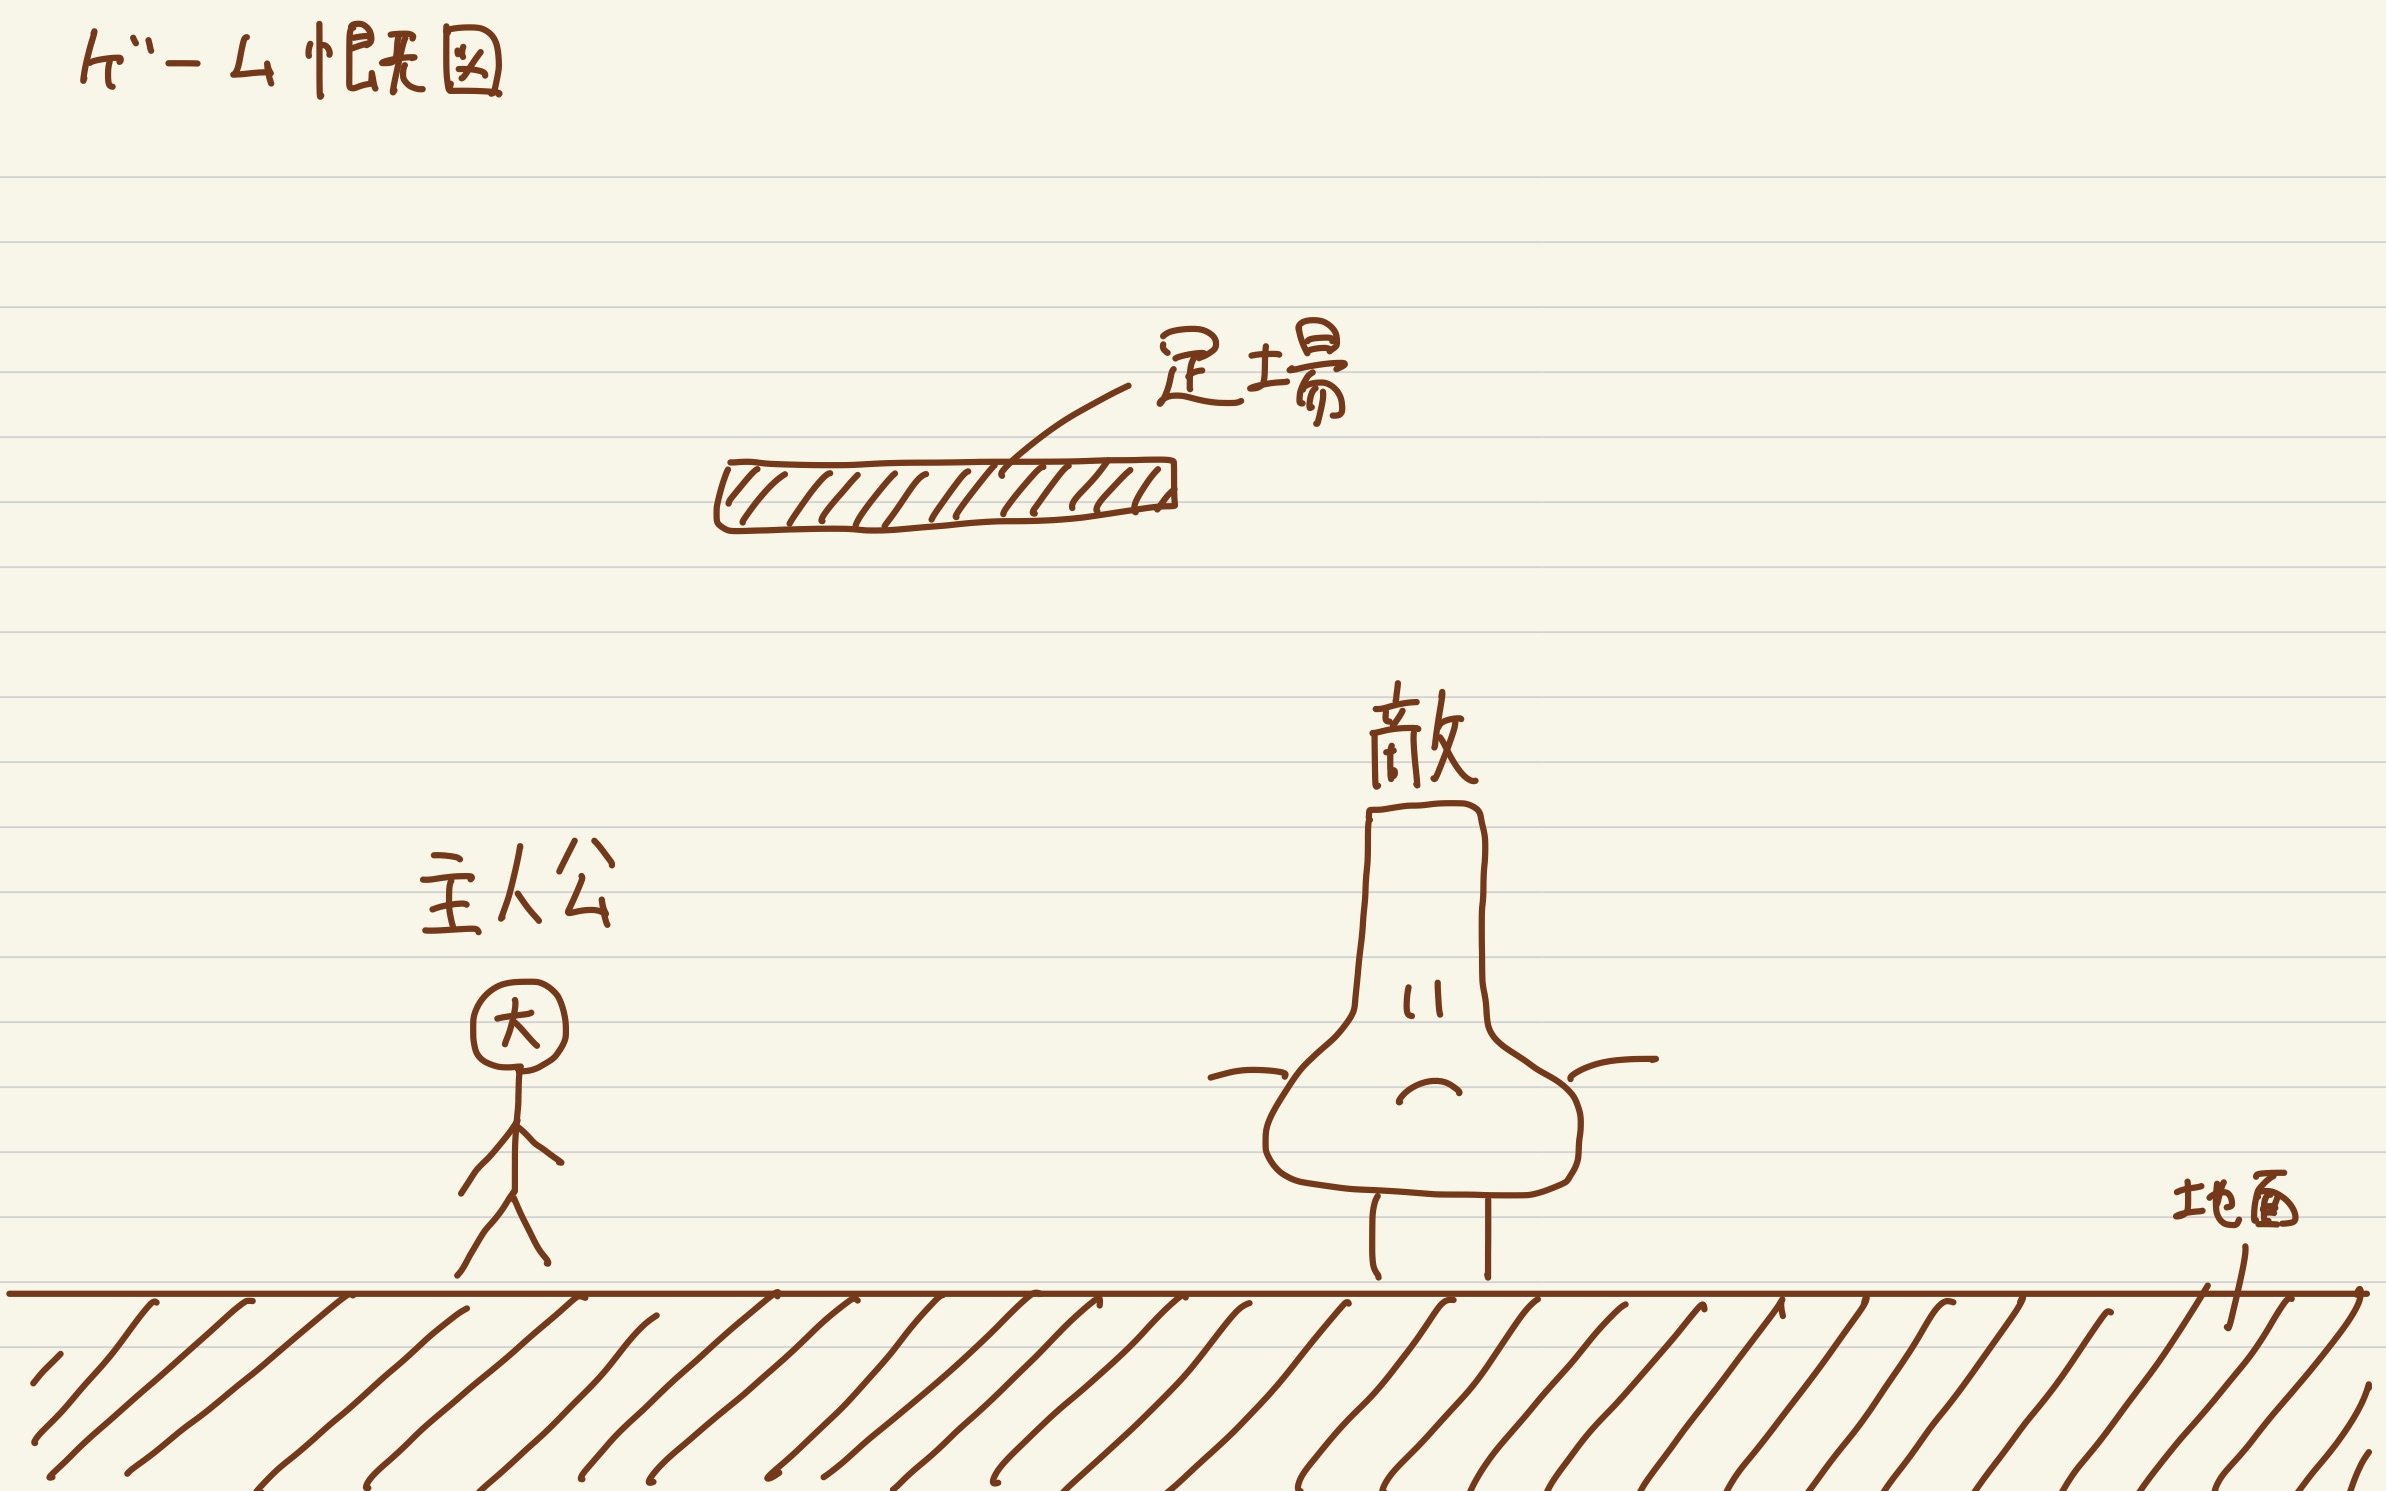
\includegraphics[width=12cm]{imags/gameGaizu.eps}
    \caption{ゲーム概図}
  \end{center}
\end{figure}

\newpage

\section{主人公-大学生}
\subsection{アクション}
\subsubsection{左右移動}

大学生が右左に動く。

\begin{figure}[htbp]
  \begin{center}
    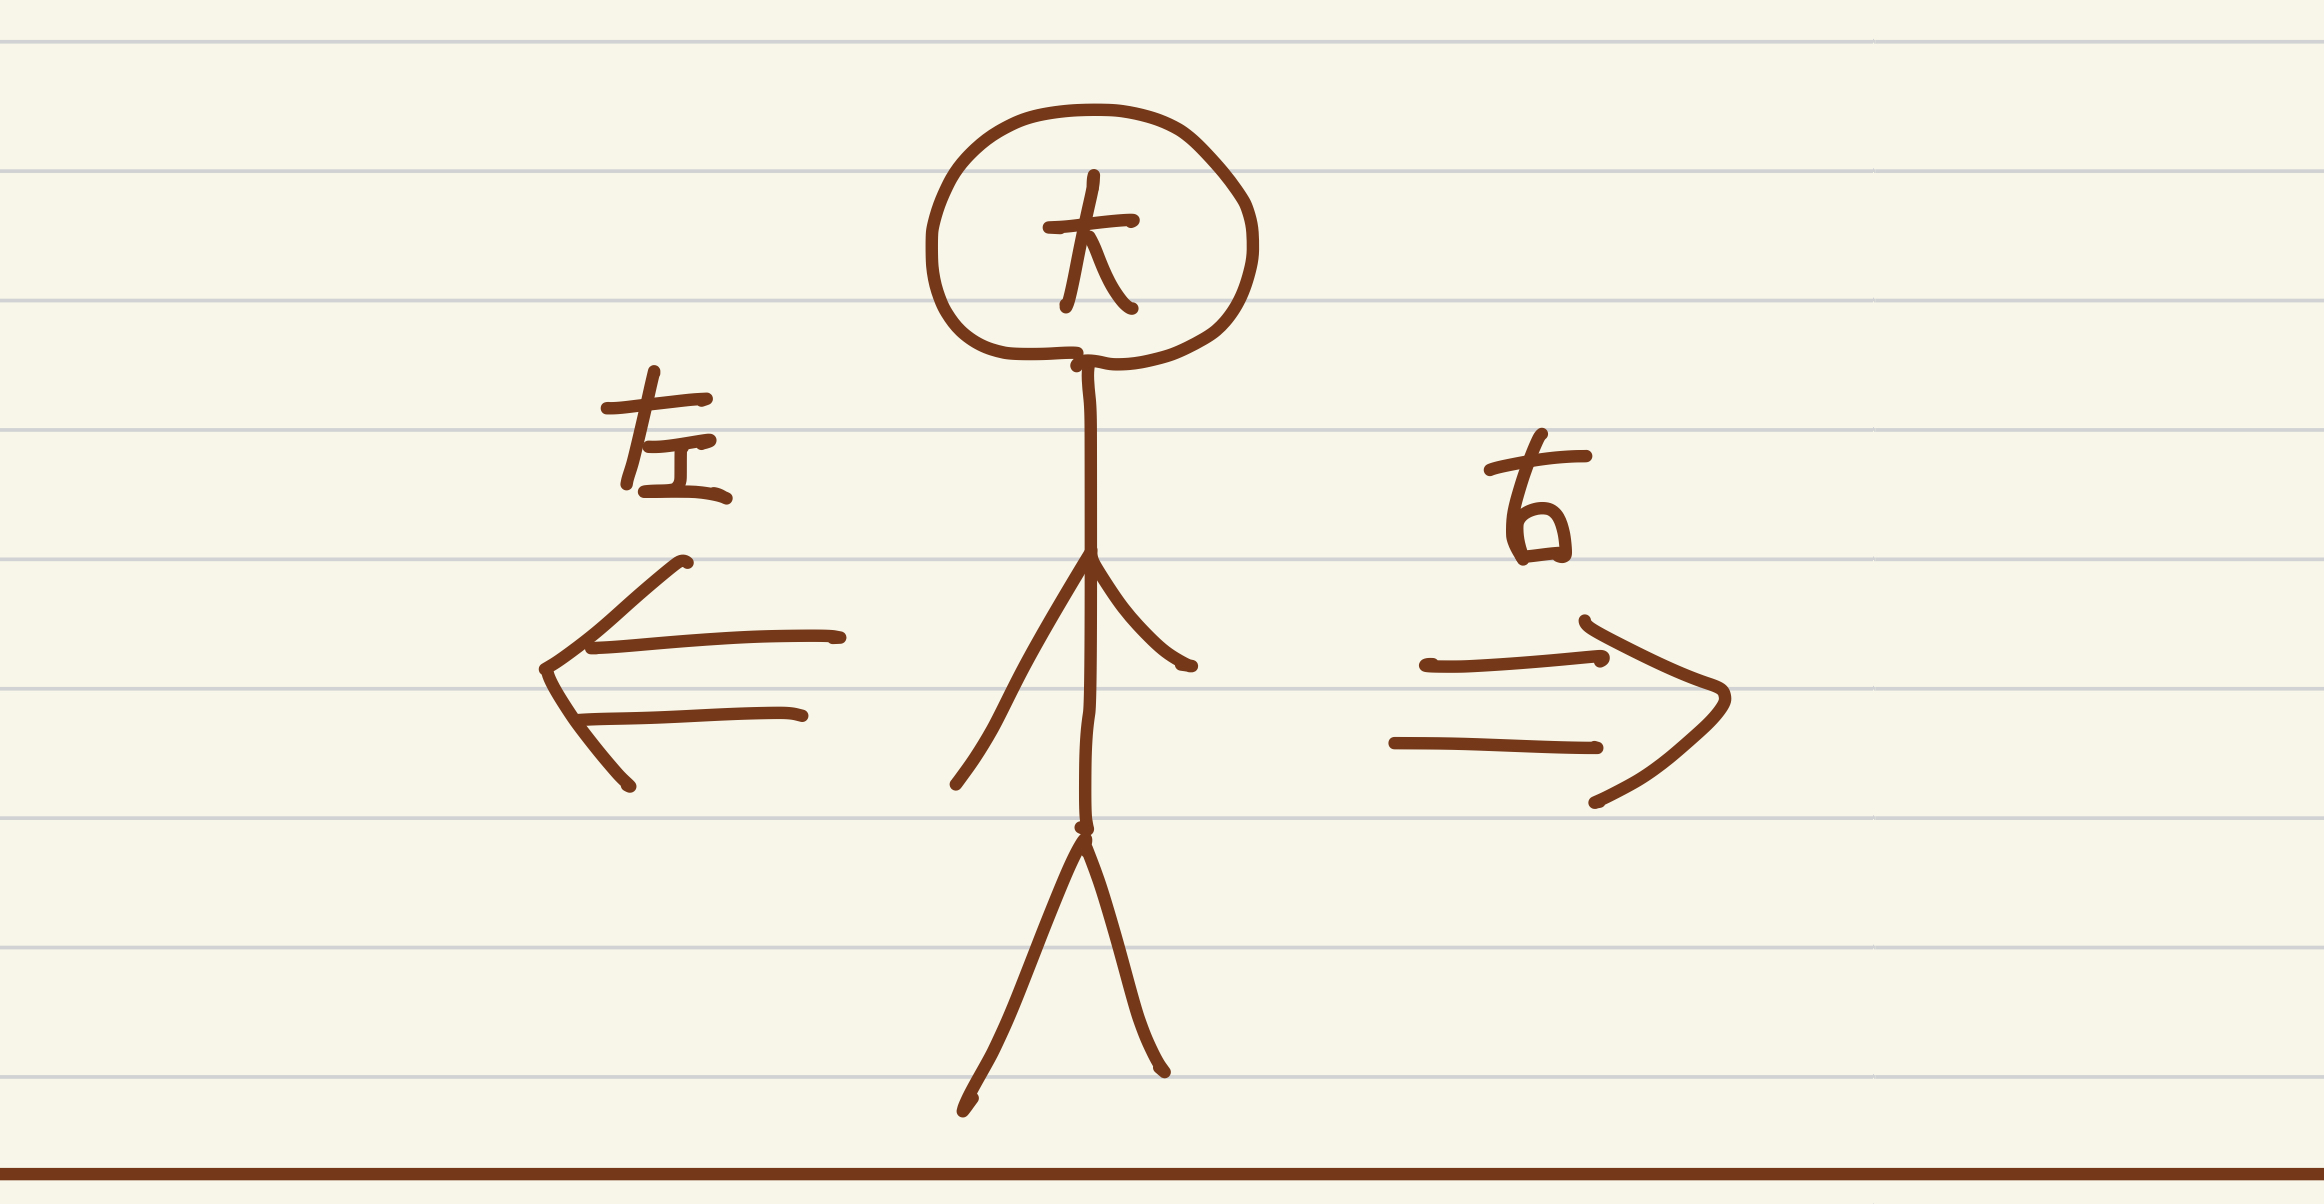
\includegraphics[width=8cm]{imags/daigakuseiSayuu.eps}
    \caption{左右に動く大学生}
  \end{center}
\end{figure}

\begin{table}[htbp]
  \centering
  \caption{PCでの左右移動のキー対応}
  \begin{tabular}{c|c}
    \hline
    動作 & 対応するキー \\
    \hline
    右に動く & 右矢印キー \\
      & Dキー \\
    \hline
    左に動く & 左矢印キー \\
      & Aキー \\
    \hline
  \end{tabular}
\end{table}

\begin{table}[htbp]
  \centering
  \caption{コントローラーでの左右移動のボタン対応}
  \begin{tabular}{c|c}
    \hline
    動作 & 対応するボタン\\
    \hline
    右に動く & 右方向ボタン \\
      & Lスティックを右に \\
    \hline
    左に動く & 左方向ボタン \\
      & Lスティックを左に \\
    \hline
  \end{tabular}
\end{table}

\newpage

\begin{figure}[htbp]
  \begin{center}
    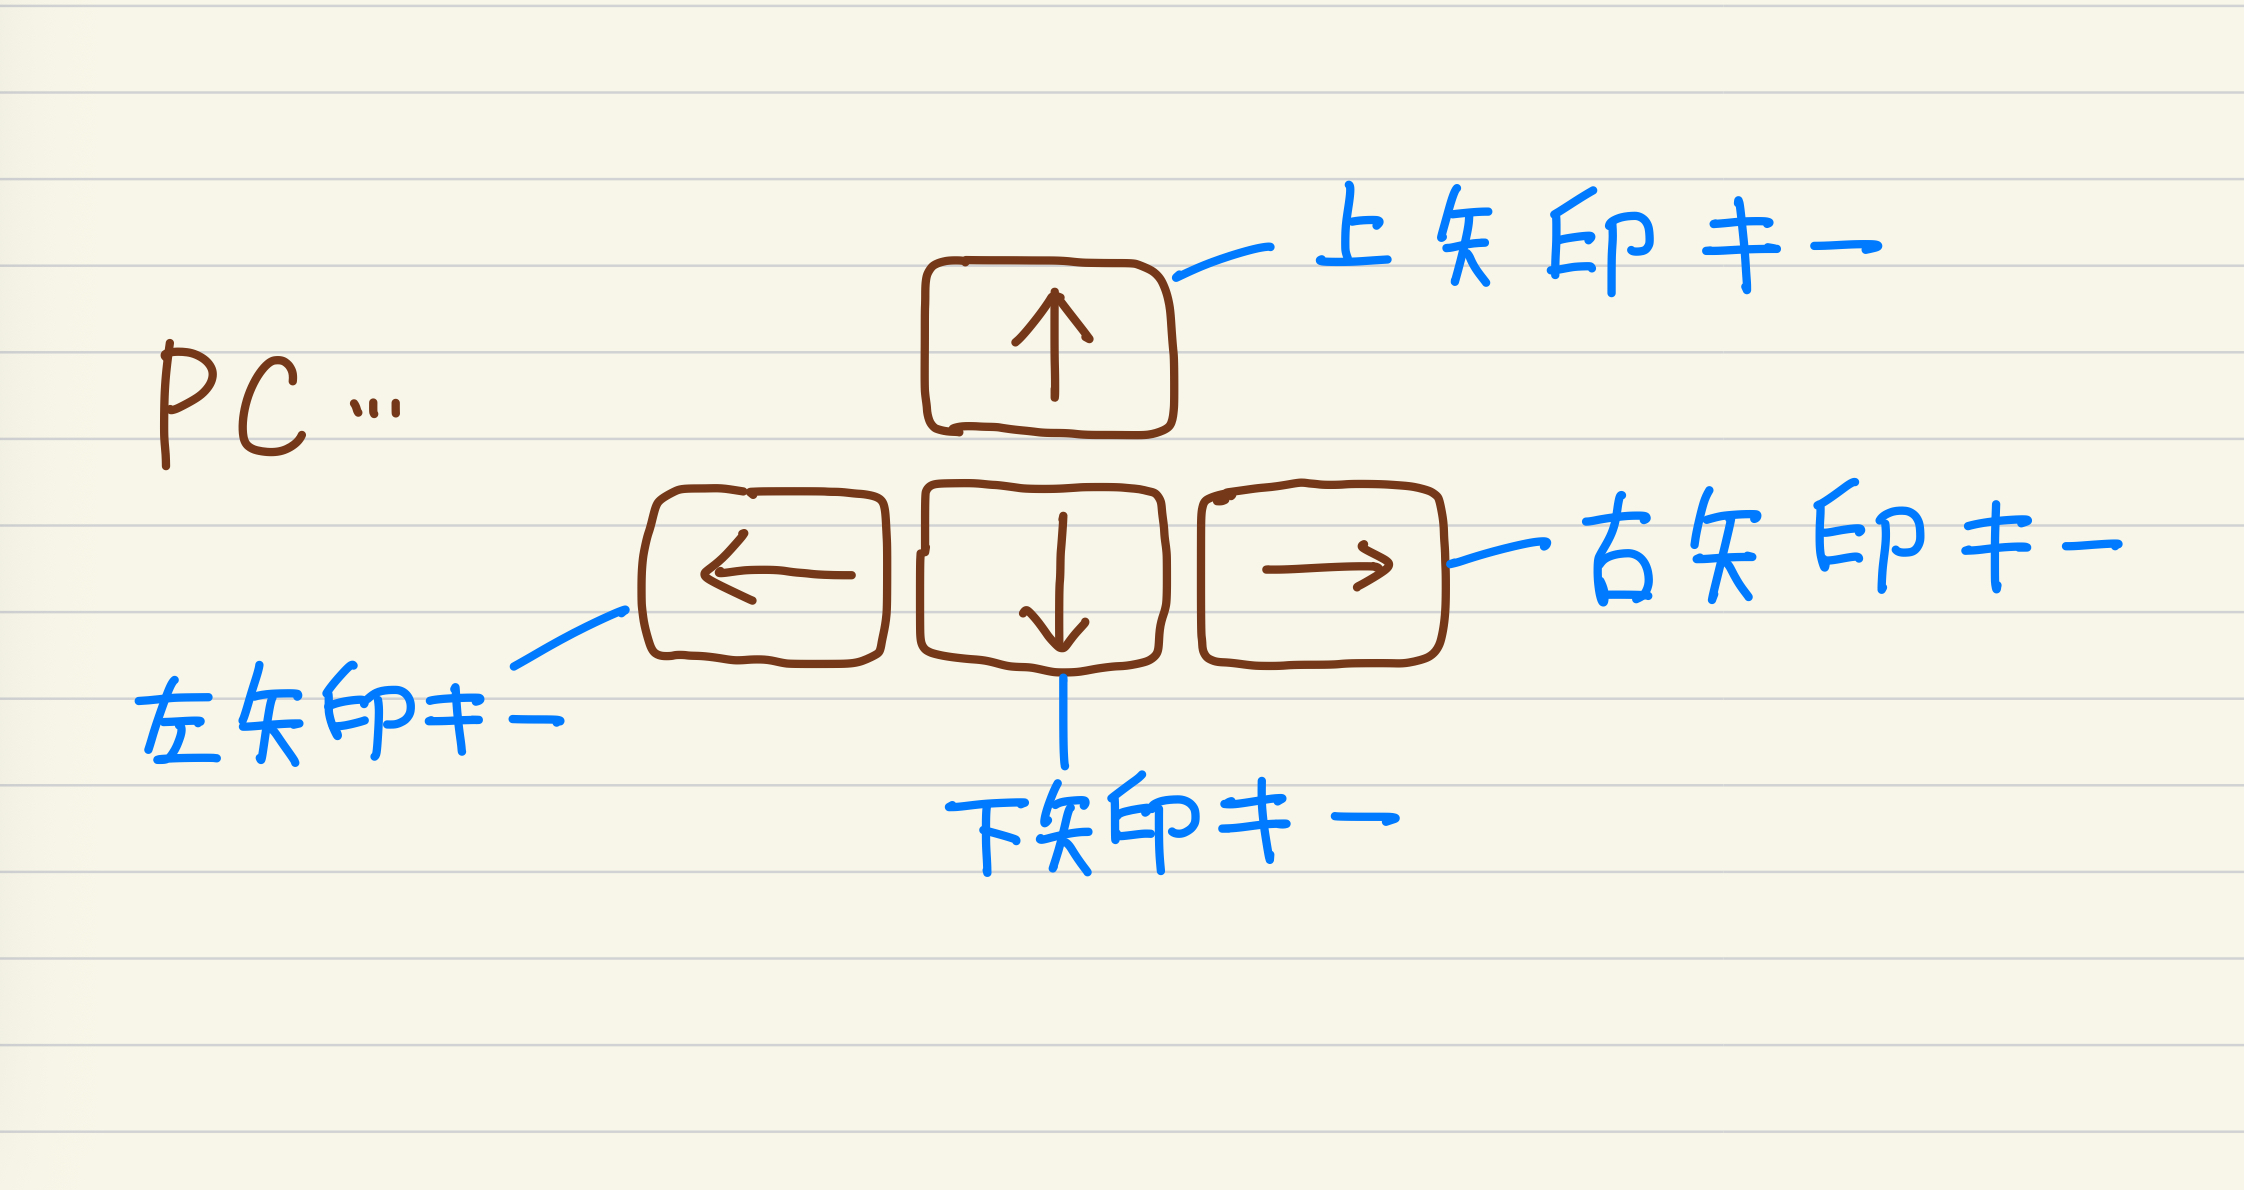
\includegraphics[width=12cm]{imags/PCYajirusiKeyDiscription.eps}
    \caption{PCの矢印キーと名前の対応}
  \end{center}
  \begin{center}
    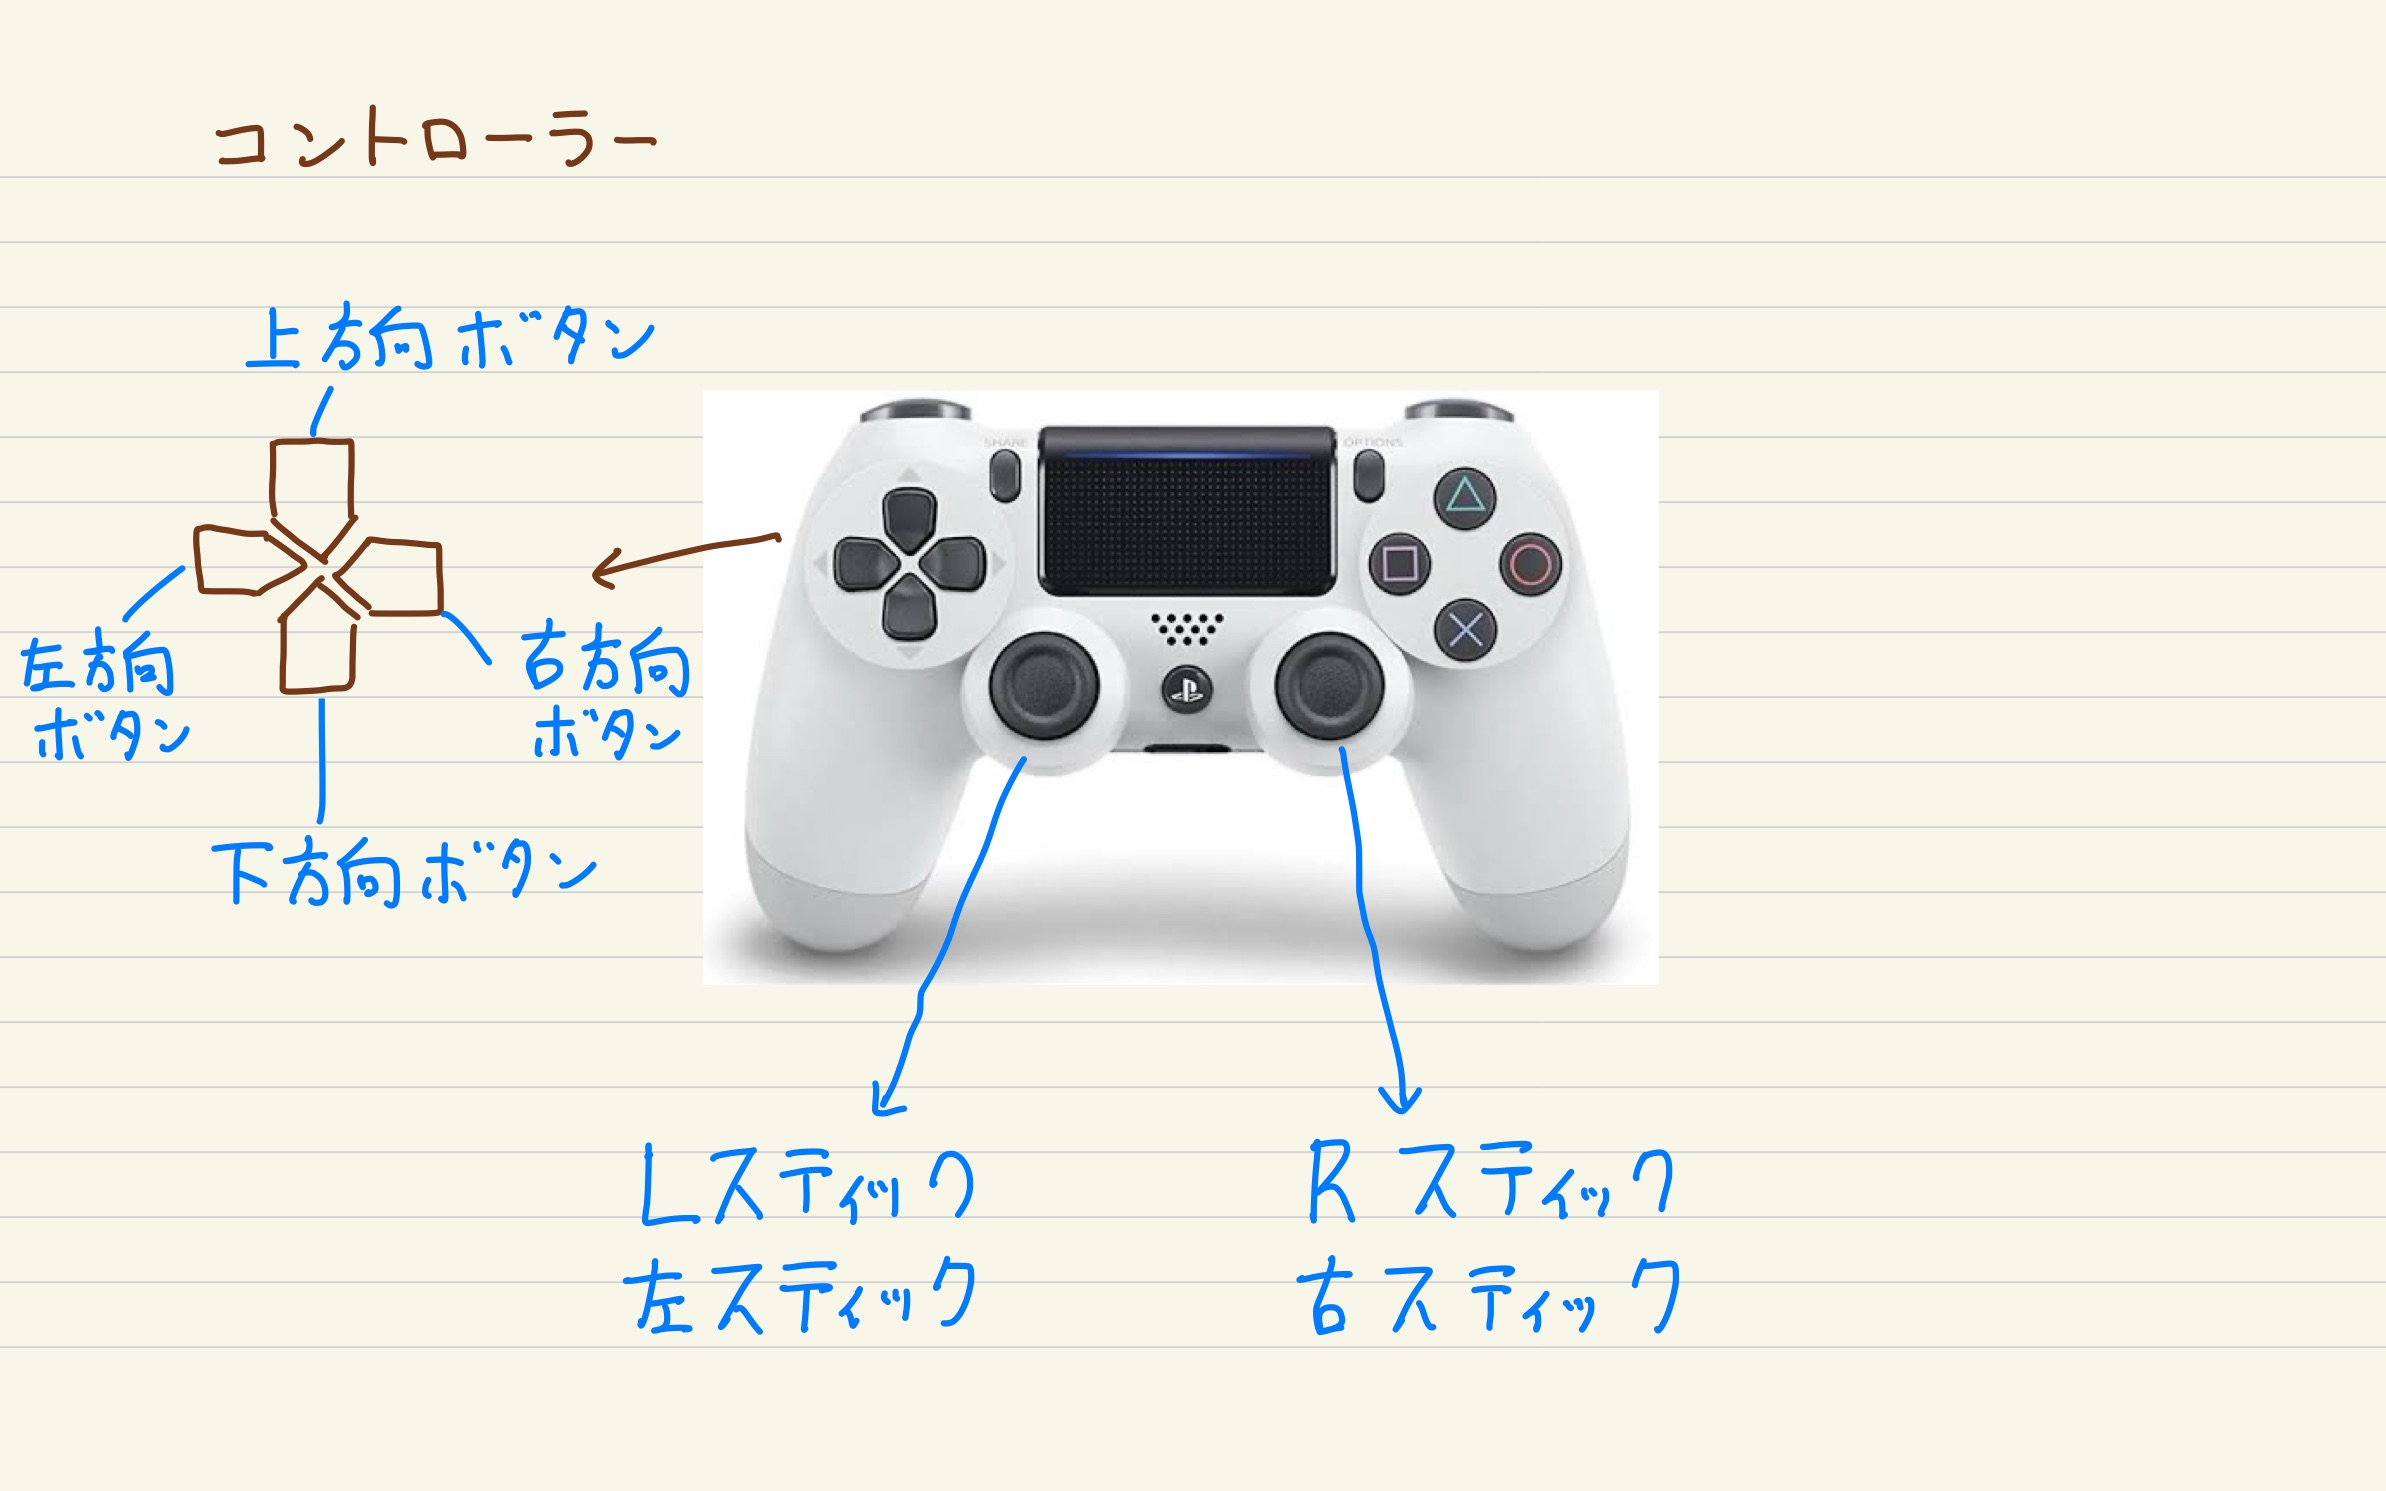
\includegraphics[width=12cm]{imags/ControllerBottunDiscription.eps}
    \caption{コントローラーのボタンと名前の対応}
  \end{center}
\end{figure}

\newpage

・左右移動-仕様
\begin{enumerate}
  \item 地面の上で左右に動く
  \item 空中で左右に動く
  \item 左右に動けない時は動かない
  \begin{enumerate}
    \item 移動方向に壁がある時
  \end{enumerate}
\end{enumerate}

\newpage

\subsubsection{ジャンプ}

ジャンプボタンを押すと、大学生が上に飛ぶ。

\begin{figure}[htbp]
  \begin{center}
    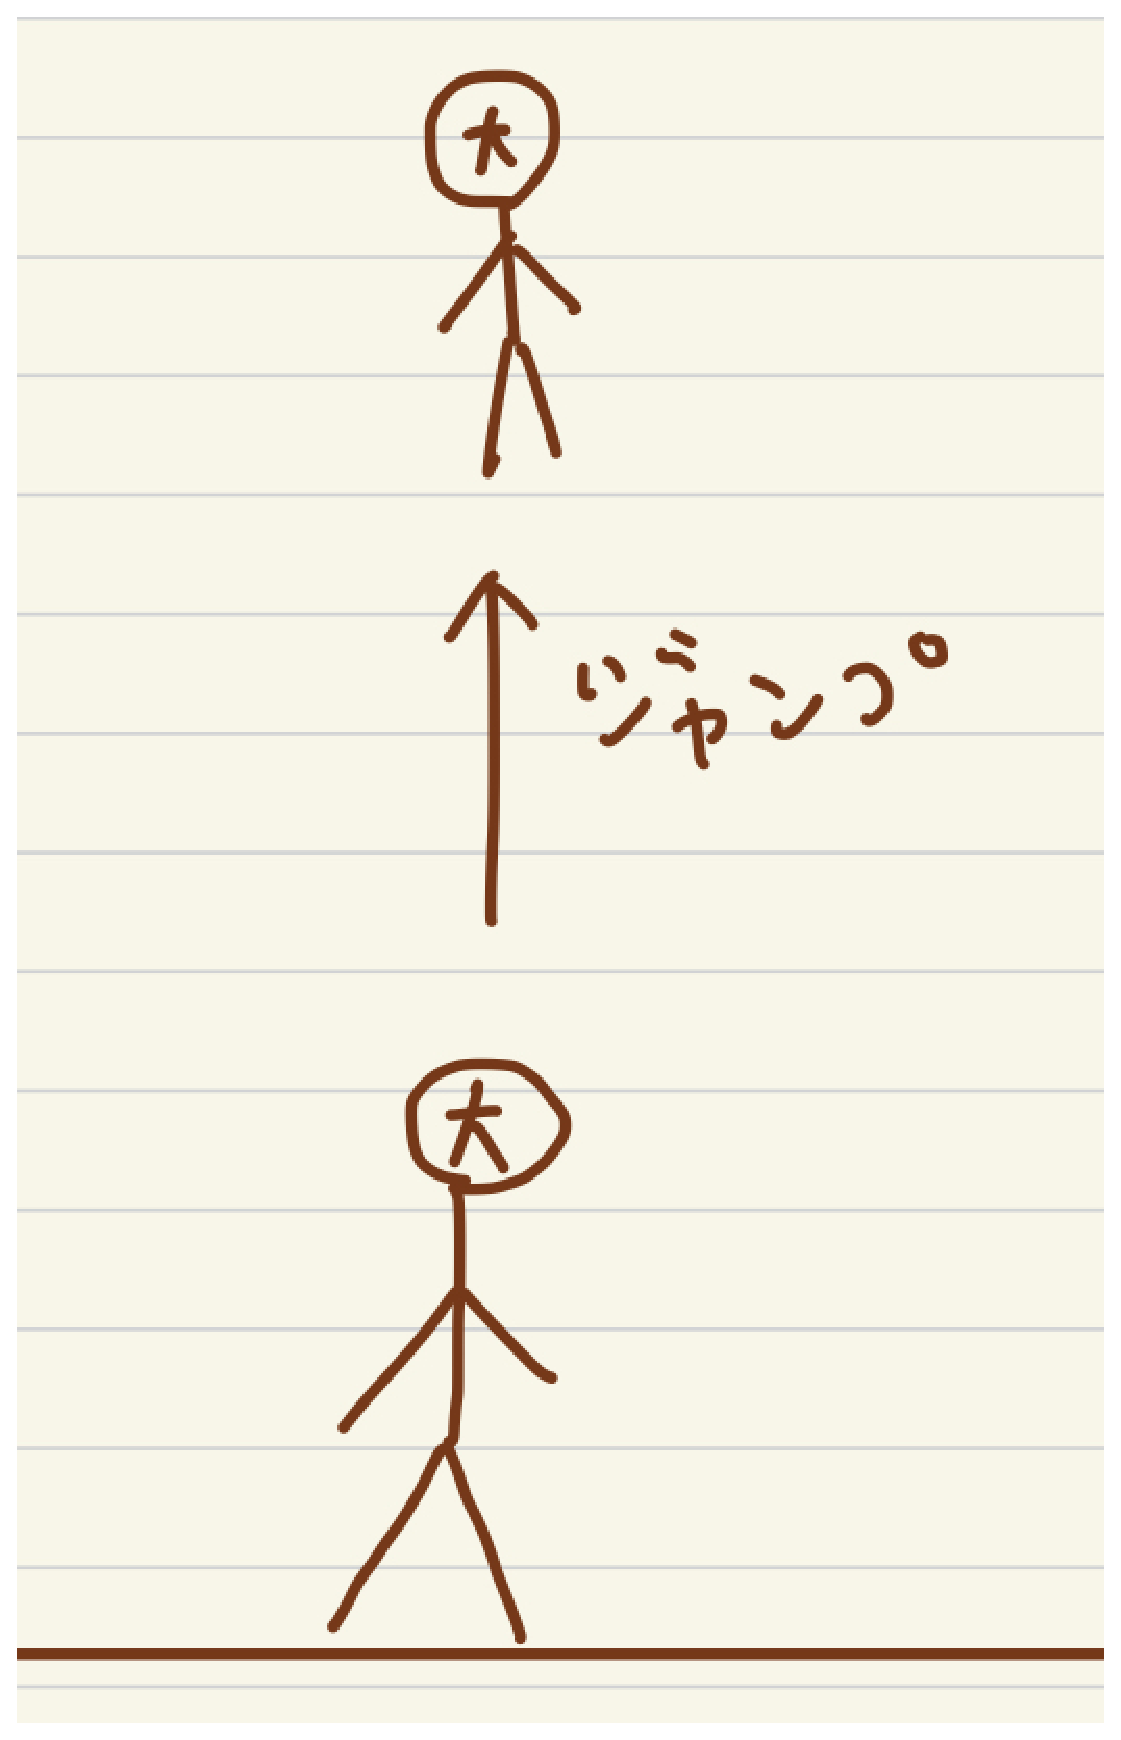
\includegraphics[height=10cm]{imags/jumpDiscription.eps}
    \caption{ジャンプする大学生}
  \end{center}
\end{figure}

\newpage

\begin{table}[htbp]
  \centering
  \caption{ジャンプボタンの対応}
  \begin{tabular}{c|c}
    \hline
    端末 & キー/ボタン \\
    \hline
    PC & 上矢印キー \\
      & Wキー \\
      & Jキー \\
    \hline
    コントローラー & Aボタン \\
      & 丸ボタン \\
      & Lスティック上入力 (要検討) \\
      \hline
  \end{tabular}
\end{table}


・Lスティック上入力について

スマブラは上入力でジャンプ

調布祭は子供が多い

ボタン押すだけに比べて実装が面倒

実装するかどうか悩む〜〜〜〜

って感じ

\vspace{1em}

・ジャンプ-仕様

\begin{enumerate}
  \item ジャンプボタンを押すと大学生が上に飛ぶ
  \item 押す長さによって飛ぶ高さが変わる
  \begin{enumerate}
    \item 短く押すと最小の高さ (要調整)でジャンプする
    \item ある程度までは、押すほど高さが伸びる
    \item 一定の高さまで上昇すると、ボタンを押しても高さが伸びなくなる
  \end{enumerate}
  \item 上に天井などがあると、ぶつかってそれ以上上昇しない
\end{enumerate}

\newpage

\subsubsection{エナドリ}

エナドリボタンを押すと、押す長さによって特定のエナドリを投げる。

押す時間の塩梅は実際にやってみて決める。

\begin{figure}[htbp]
  \begin{center}
    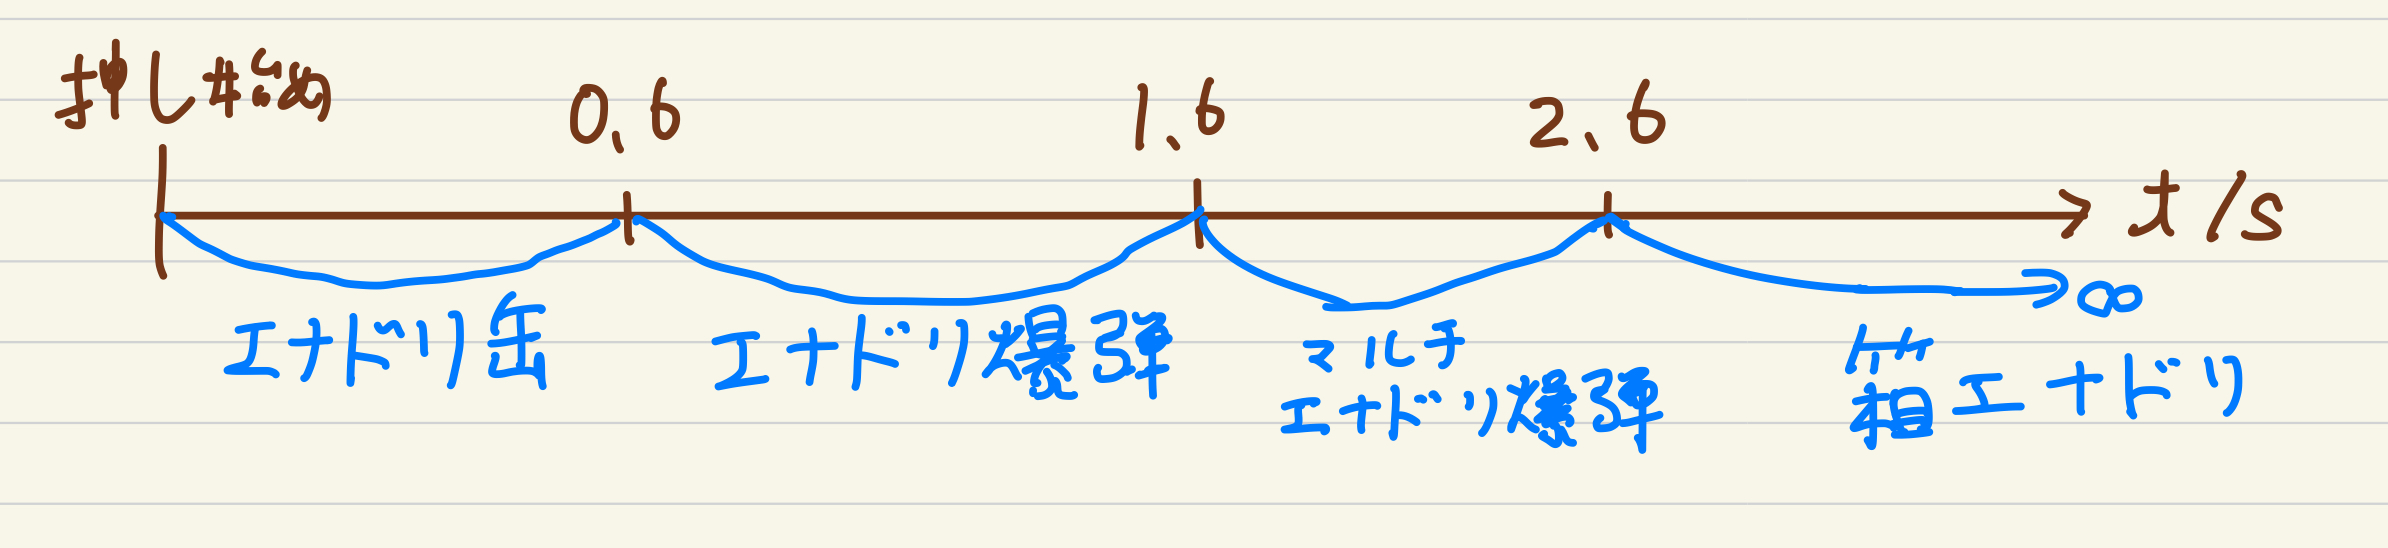
\includegraphics[width=12cm]{imags/enadoriPushDiscription.eps}
    \caption{エナドリボタンを押す長さで、投げるものが変わる}
  \end{center}
\end{figure}


\begin{table}[htbp]
  \caption{エナドリボタンと操作割り当て}
  \centering
  \begin{tabular}{c|c}
    \hline
    端末 & 割り当て \\
    \hline
    PC & スペース \\
      & Xキー \\
      & Kキー \\
    \hline
    コントローラー & R1 \\
      & R2 \\
      & L1 \\
      & L2 \\
      & Xボタン \\
      & Bボタン \\
      & 三角ボタン \\
      & バツボタン \\
    \hline
  \end{tabular}
\end{table}

\newpage

・エナドリ缶

エナドリボタンを0〜0.6秒 (要調整) 押すと、エナドリ缶を投げる。

\begin{figure}[htbp]
  \begin{center}
    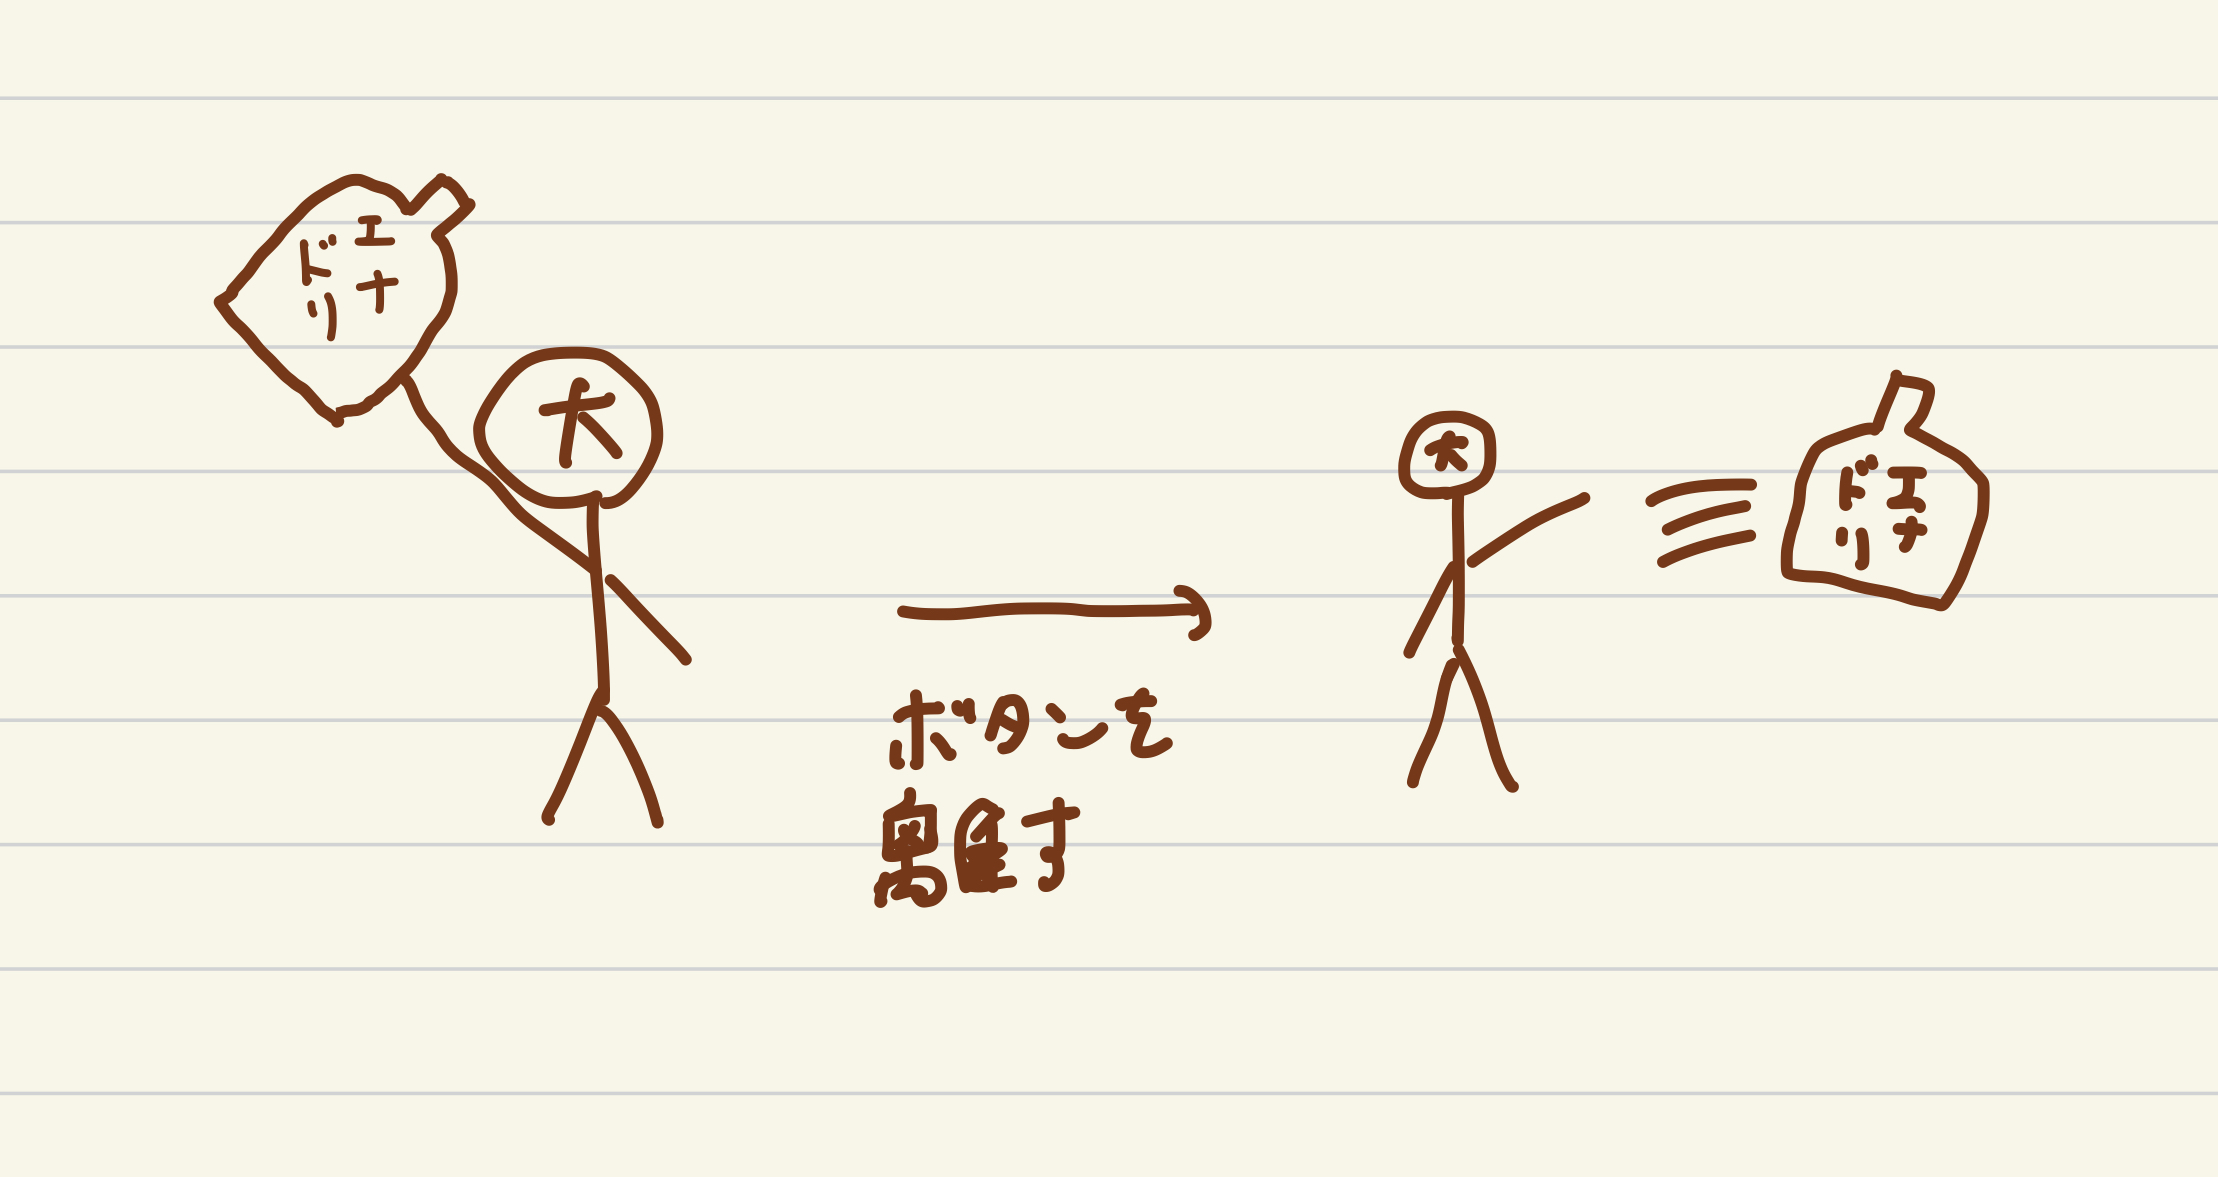
\includegraphics[width=12cm]{imags/enadoriKan.eps}
    \caption{エナドリ缶を投げる大学生}
  \end{center}
\end{figure}

\newpage

・エナドリ缶の仕様

\begin{enumerate}
  \item 左右に投げられる
  \item 投げたら、水平に飛んでいく
  \begin{figure}[htbp]
    \begin{center}
      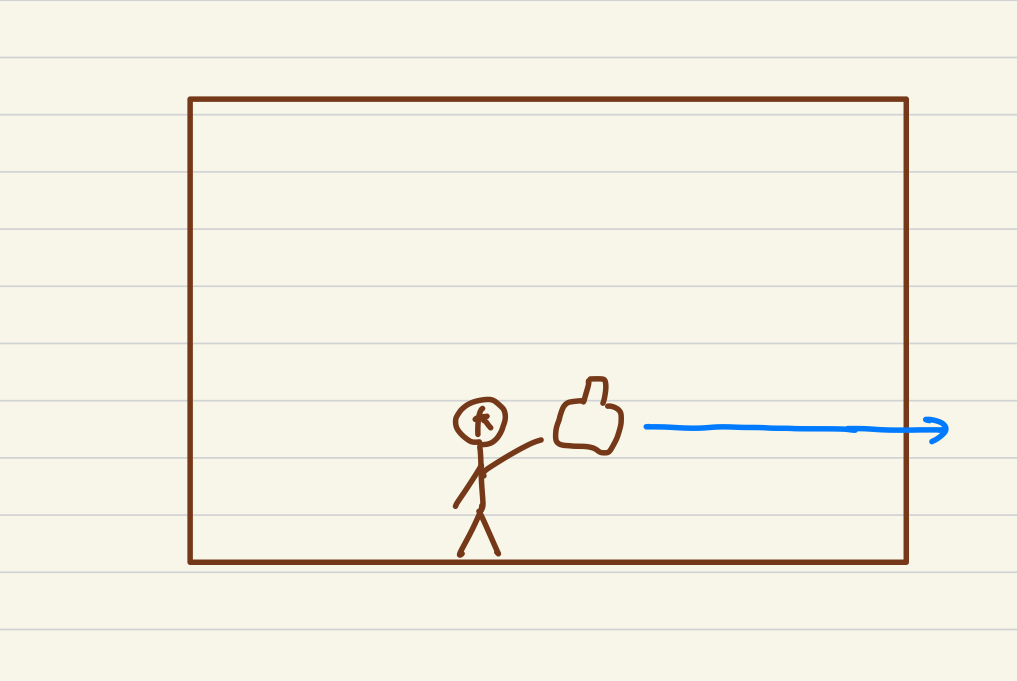
\includegraphics[width=8cm]{imags/enadoriKidou.eps}
      \caption{エナドリ缶の軌道}
    \end{center}
  \end{figure}
  \item 画面の端までいったら消える
  \item 敵や、当たり判定のあるギミックに当たると、敵にダメージを与えて消える
  \begin{figure}[htbp]
    \begin{center}
      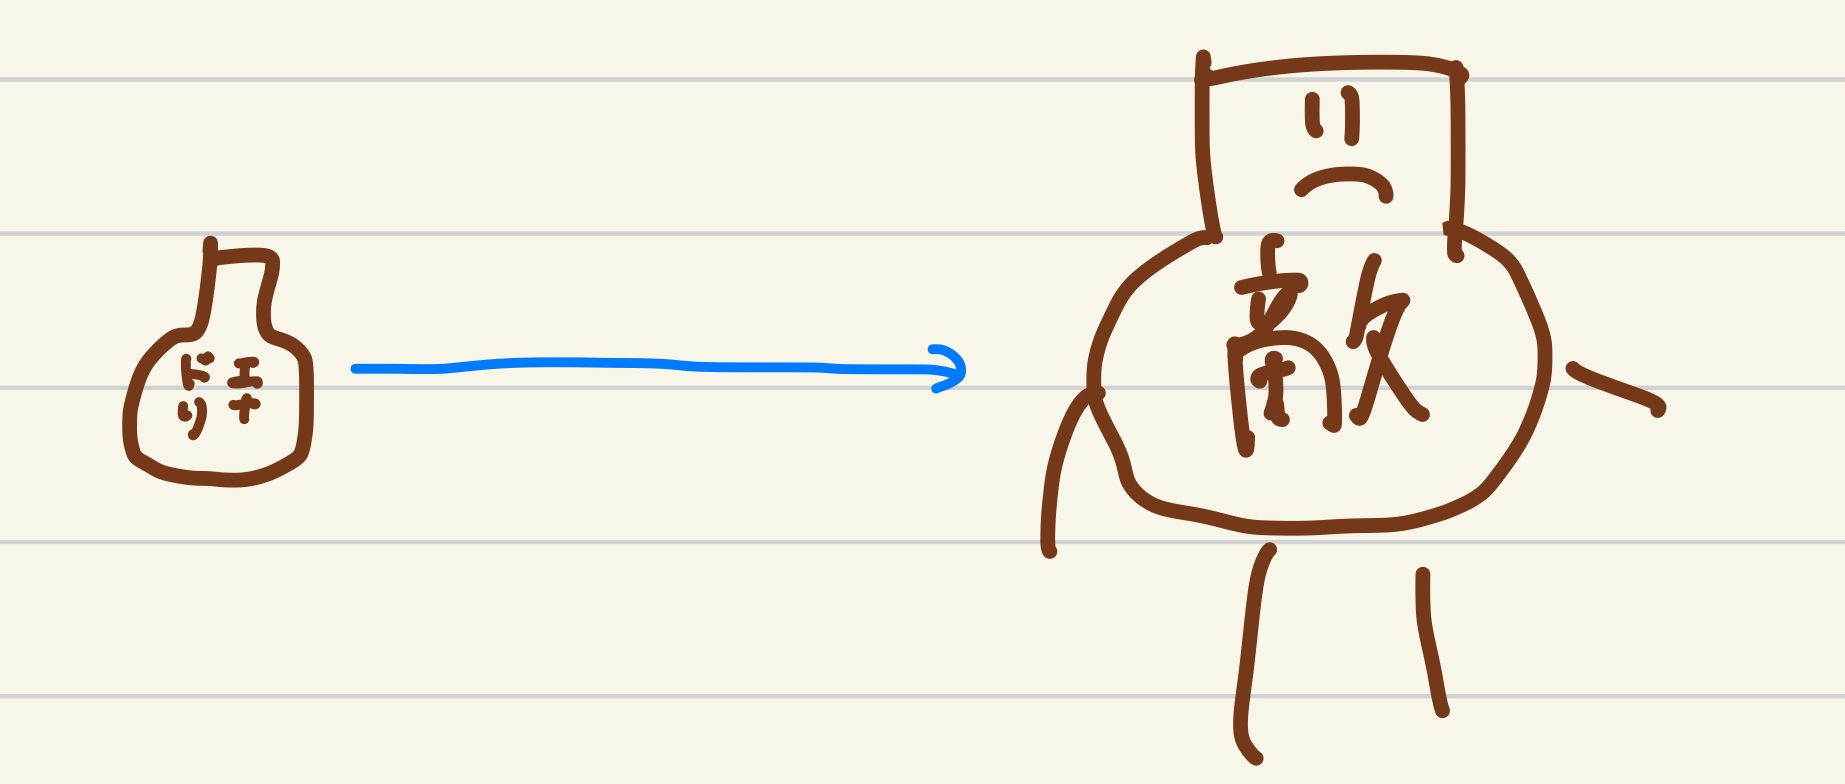
\includegraphics[width=8cm]{imags/enadoriKanTeki.eps}
      \caption{敵に当たるエナドリ缶}
    \end{center}
  \end{figure}

  \newpage
  \item エナドリボタンを押した回数だけエナドリ缶が出る
  \begin{figure}[htbp]
    \begin{center}
      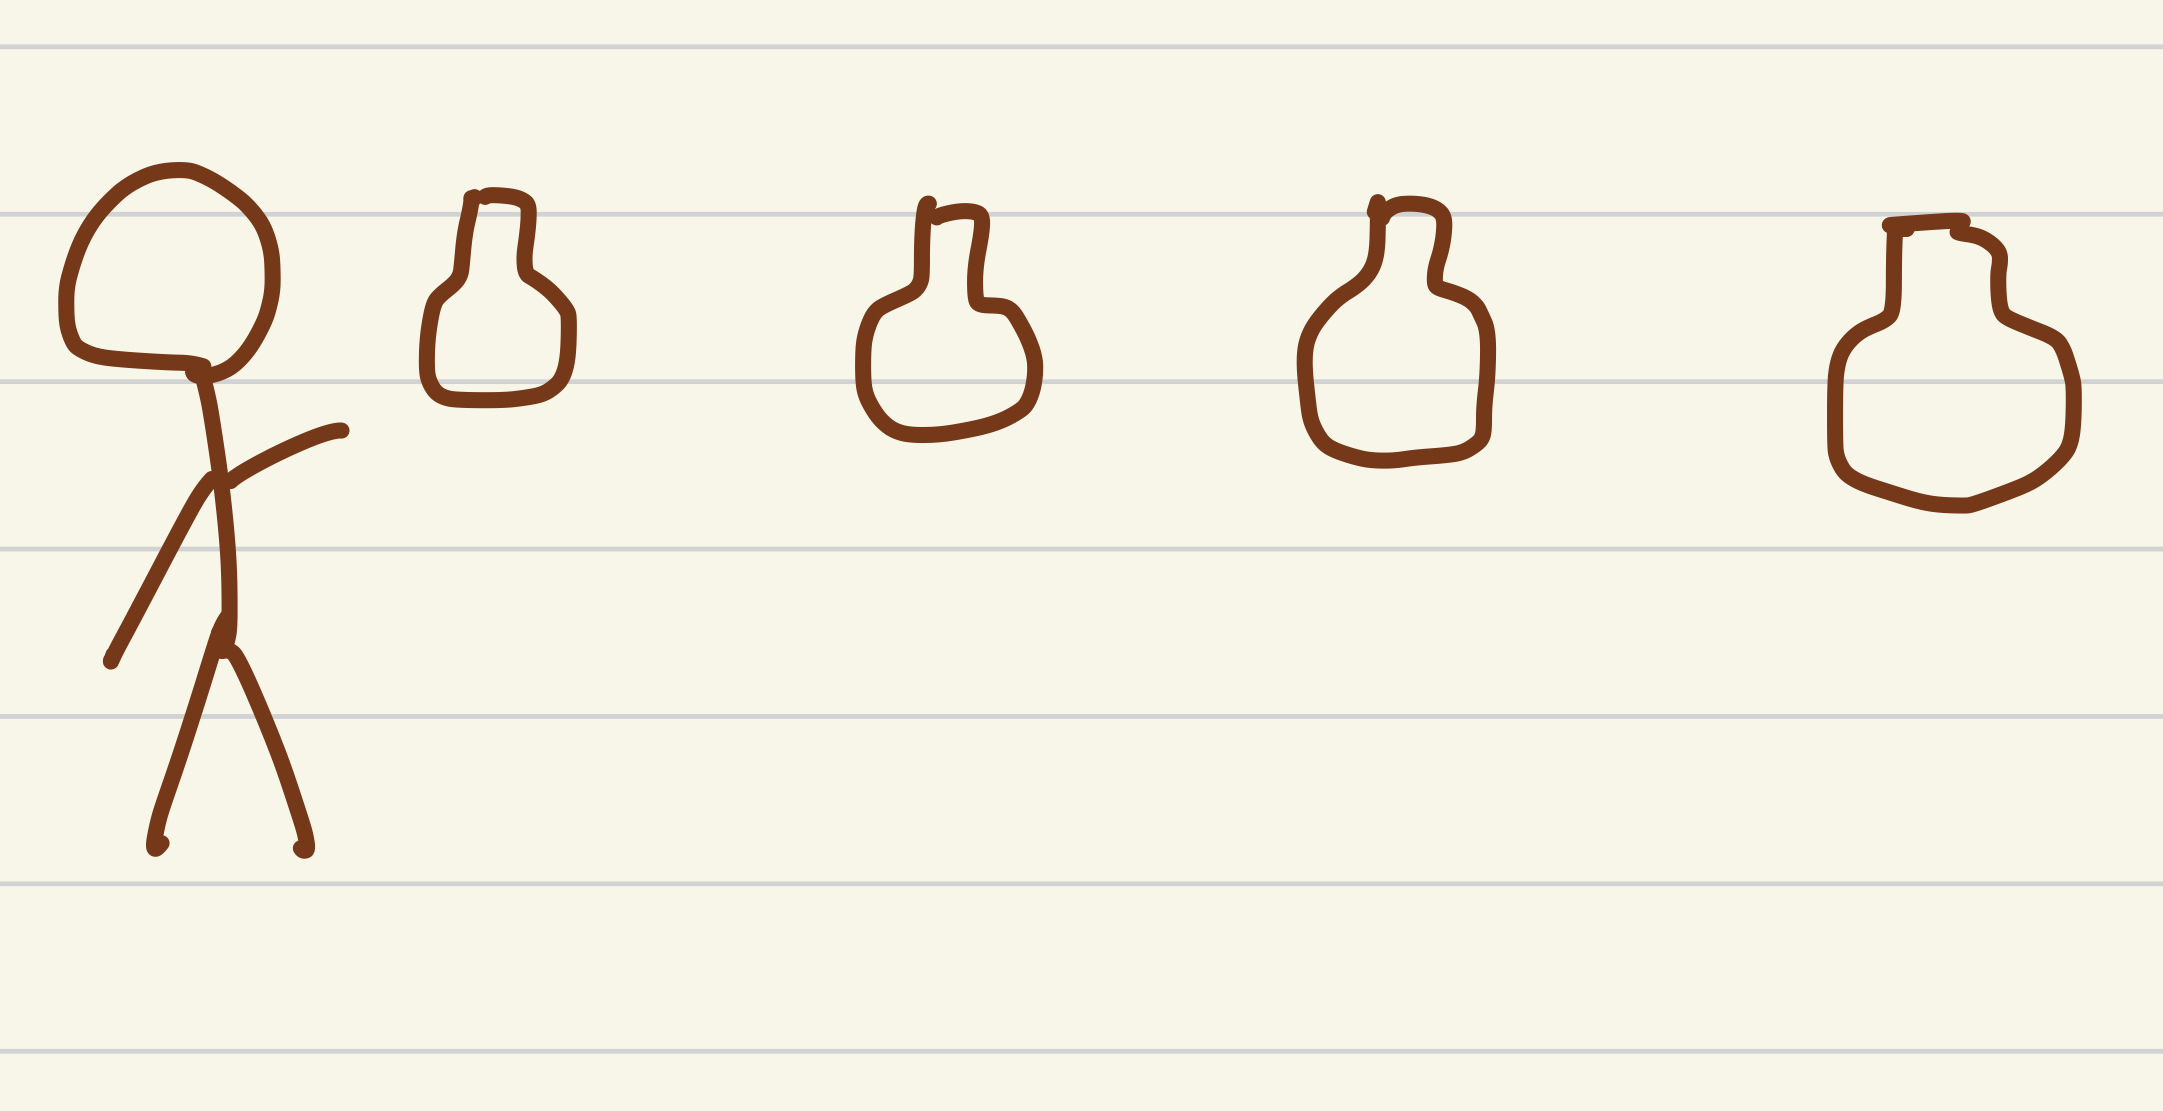
\includegraphics[width=8cm]{imags/enadoriKanMany.eps}
      \caption{エナドリ缶をたくさん投げる主人公}
    \end{center}
  \end{figure}
\end{enumerate}

\newpage

・エナドリ爆弾

エナドリボタンを0.6〜1.6秒 (要調整) 押すと、大学生がエナドリ爆弾を投げる

\begin{figure}[htbp]
  \begin{center}
    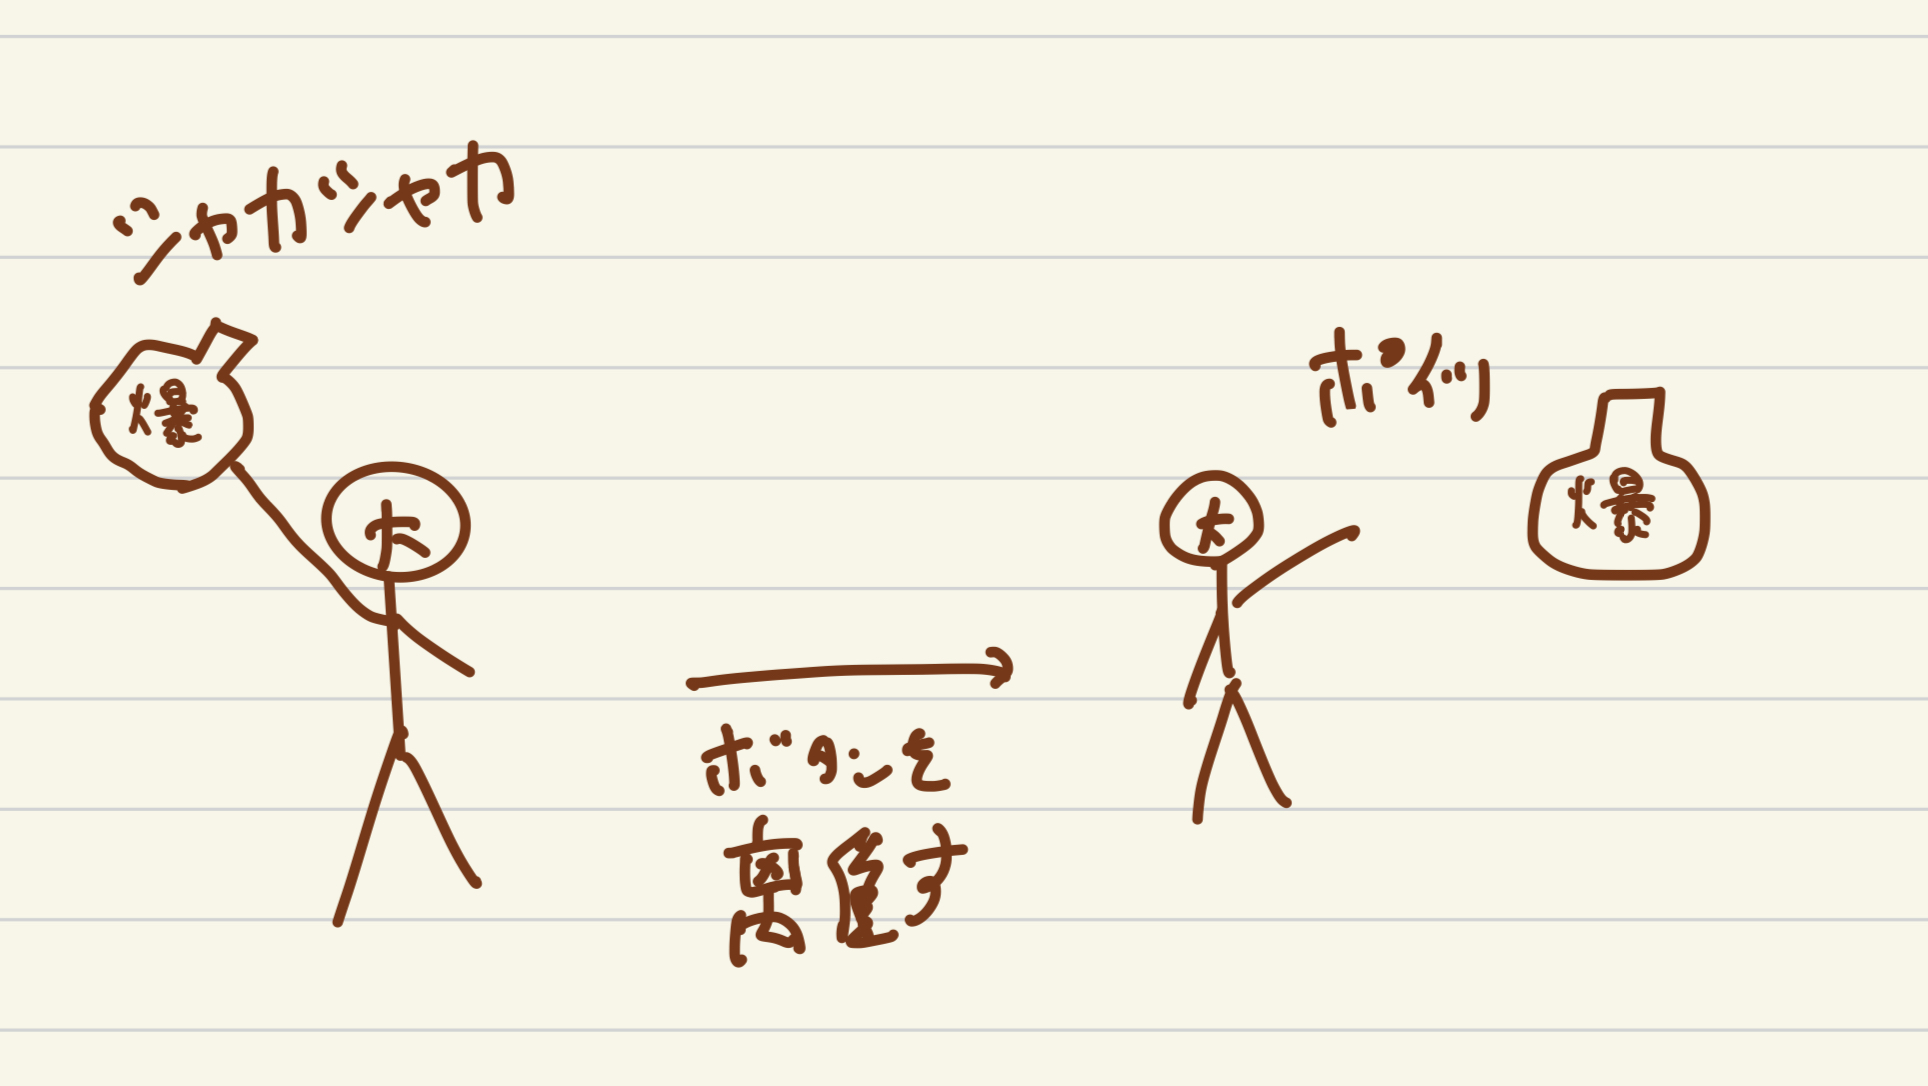
\includegraphics[width=12cm]{imags/enadoriBakudan.eps}
    \caption{エナドリ爆弾を投げる大学生}
  \end{center}
\end{figure}

・エナドリ爆弾の仕様

\begin{enumerate}
  \item 左右に投げられる
  \item エナドリ爆弾はちょっと落ちながら飛んでいく
  \begin{figure}[htbp]
    \begin{center}
      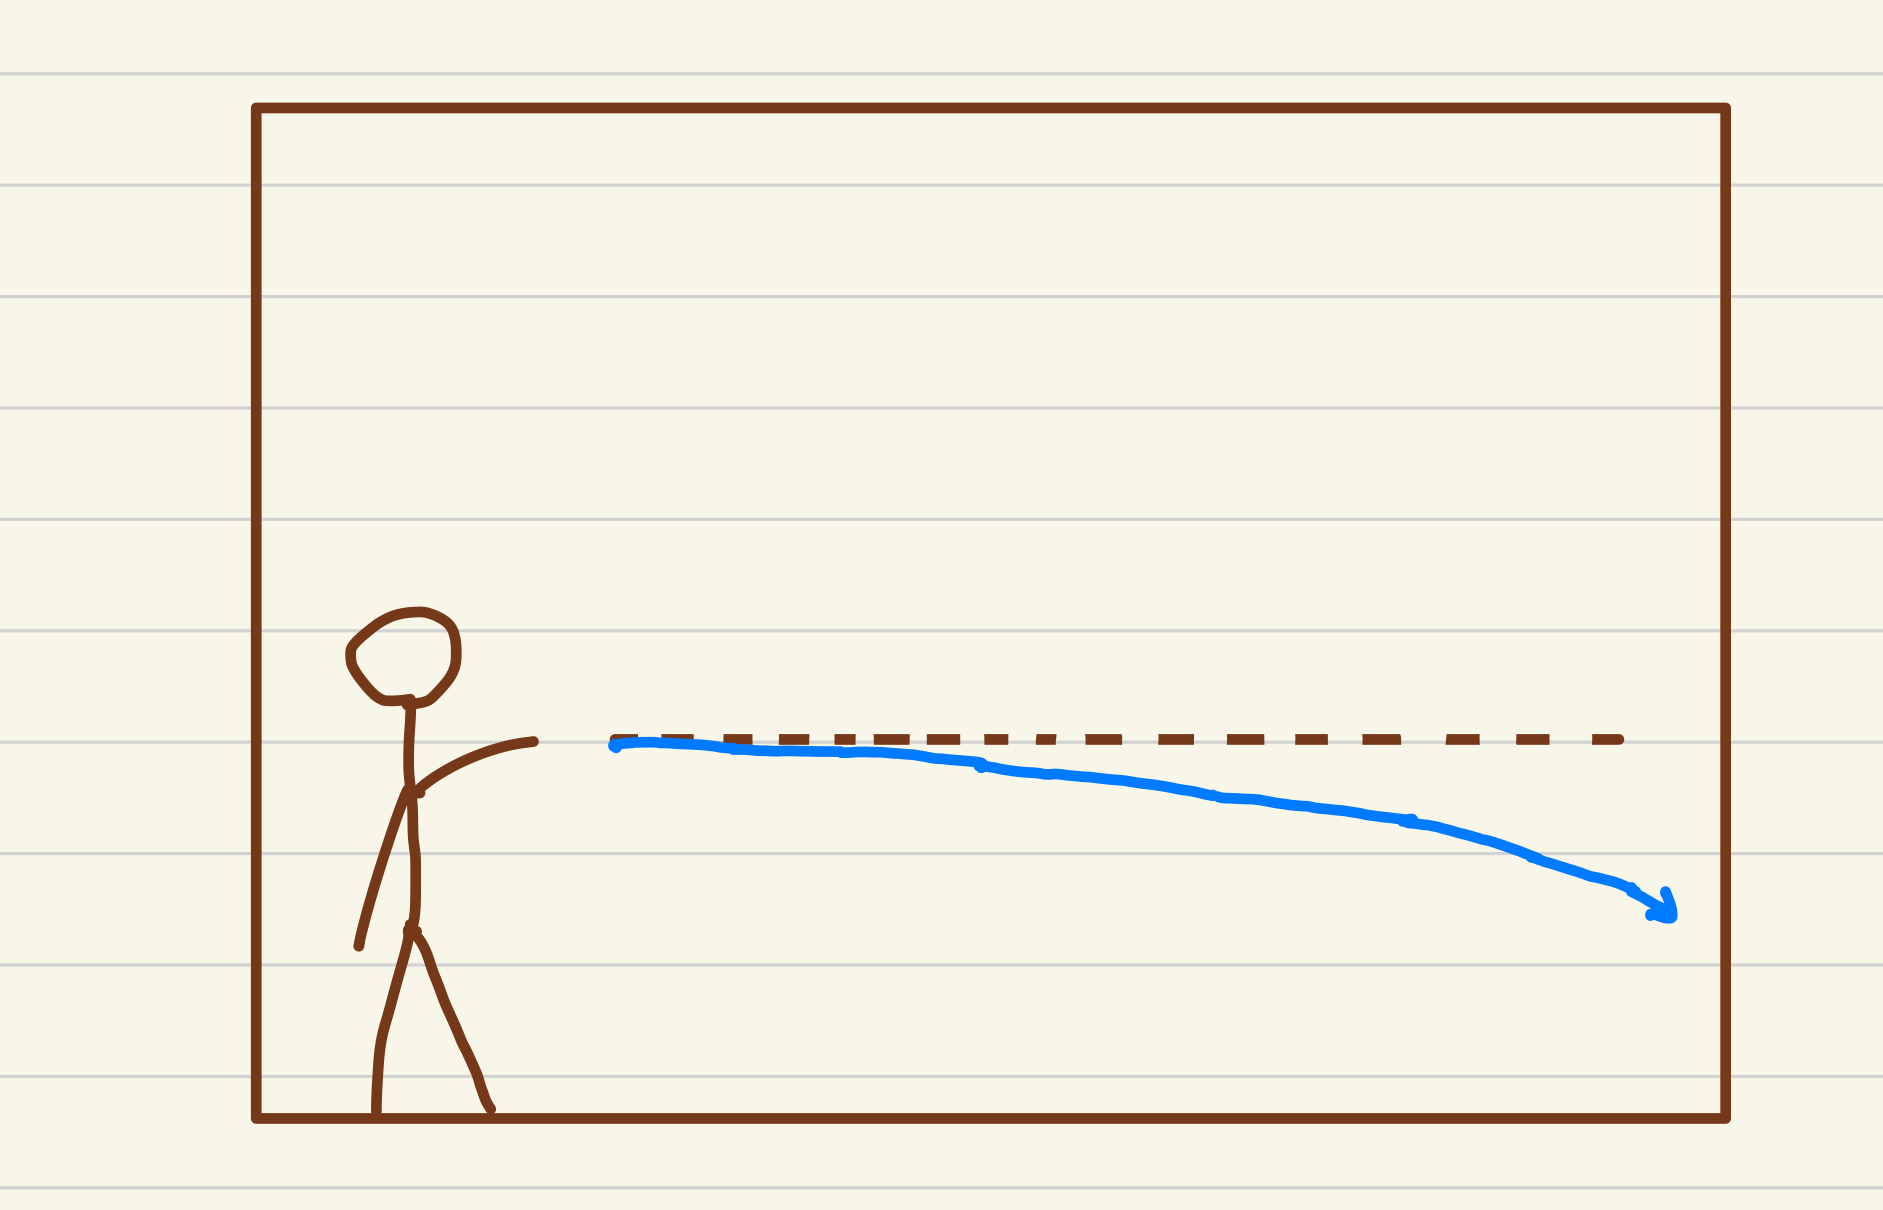
\includegraphics[width=8cm]{imags/enadoriBakudanKidou.eps}
    \end{center}
    \caption{エナドリ爆弾の軌道}
  \end{figure}

  \item 敵や当たり判定のあるギミックに当たると、爆発する
  \begin{enumerate}
    \item 敵等に接触した瞬間に爆発する
    \item 壁は貫通する (壁にあたっても爆発しない)
    \item 爆発は、敵やギミックにダメージを与える
  \end{enumerate}
  \begin{figure}[htbp]
    \begin{center}
      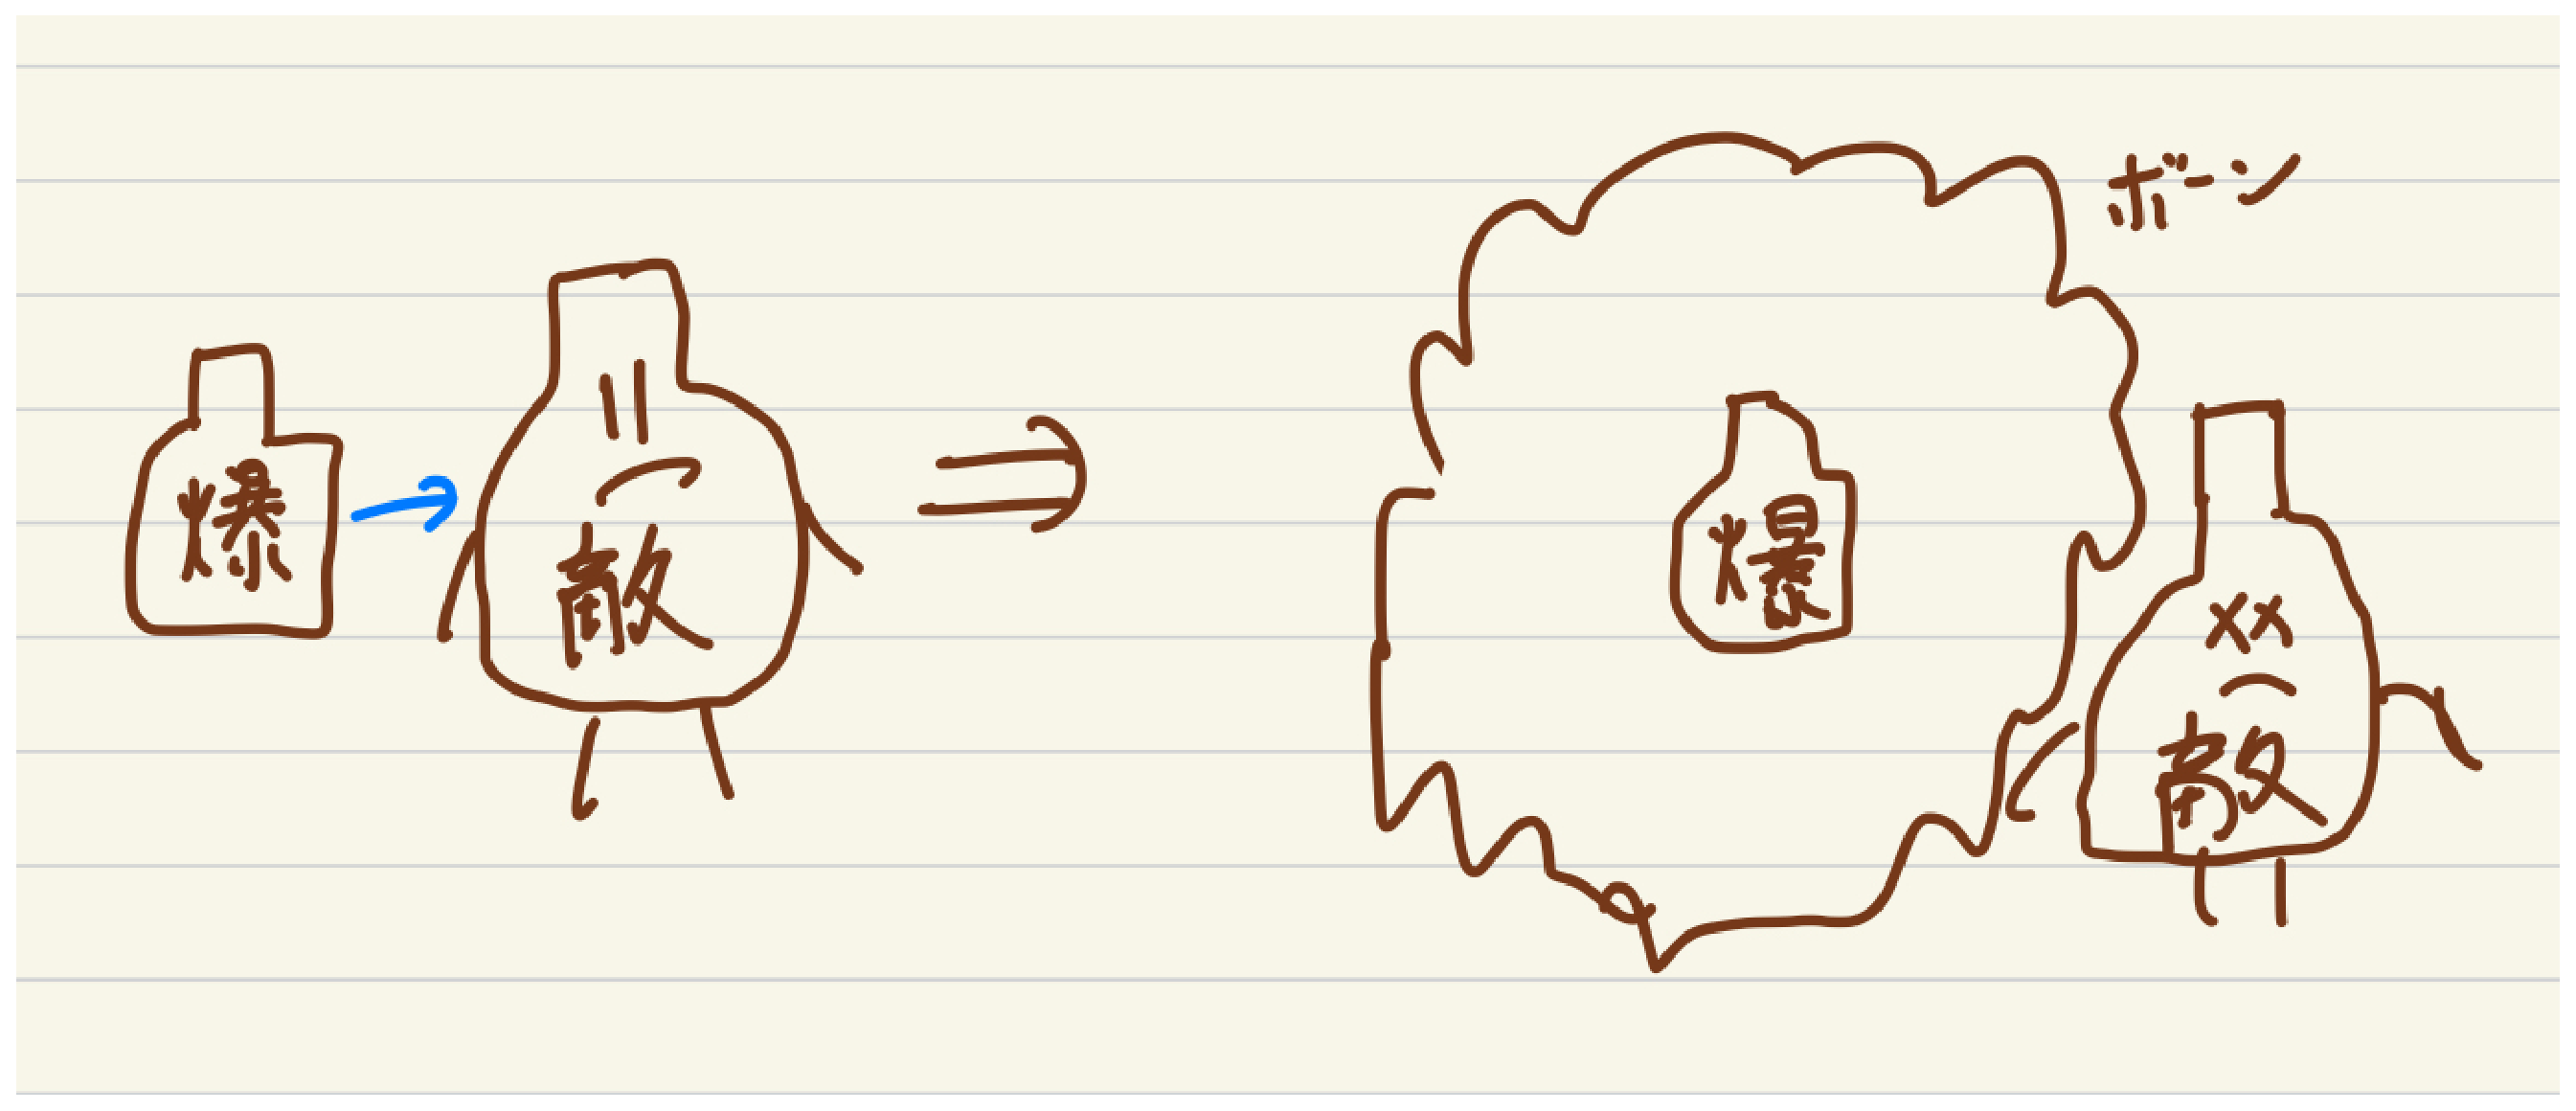
\includegraphics[width=12cm]{imags/enadoriBakudanBakuhatu.eps}
      \caption{爆発するエナドリ爆弾}
    \end{center}
  \end{figure}

  \item エナドリ爆弾は、画面の中に何個でも出せる (画面の中で個数制限はない)

  \item エナドリ爆弾を投げられる間、移動速度が90\%になる

  (エナドリボタンを押し始めてから0.6〜1.6秒で、何も投げてない時)
\end{enumerate}

\newpage

・マルチエナドリ爆弾

エナドリボタン1.6〜2.6秒で、エナドリ爆弾を3個 (要調整) 投げる。

\begin{figure}[htbp]
  \begin{center}
    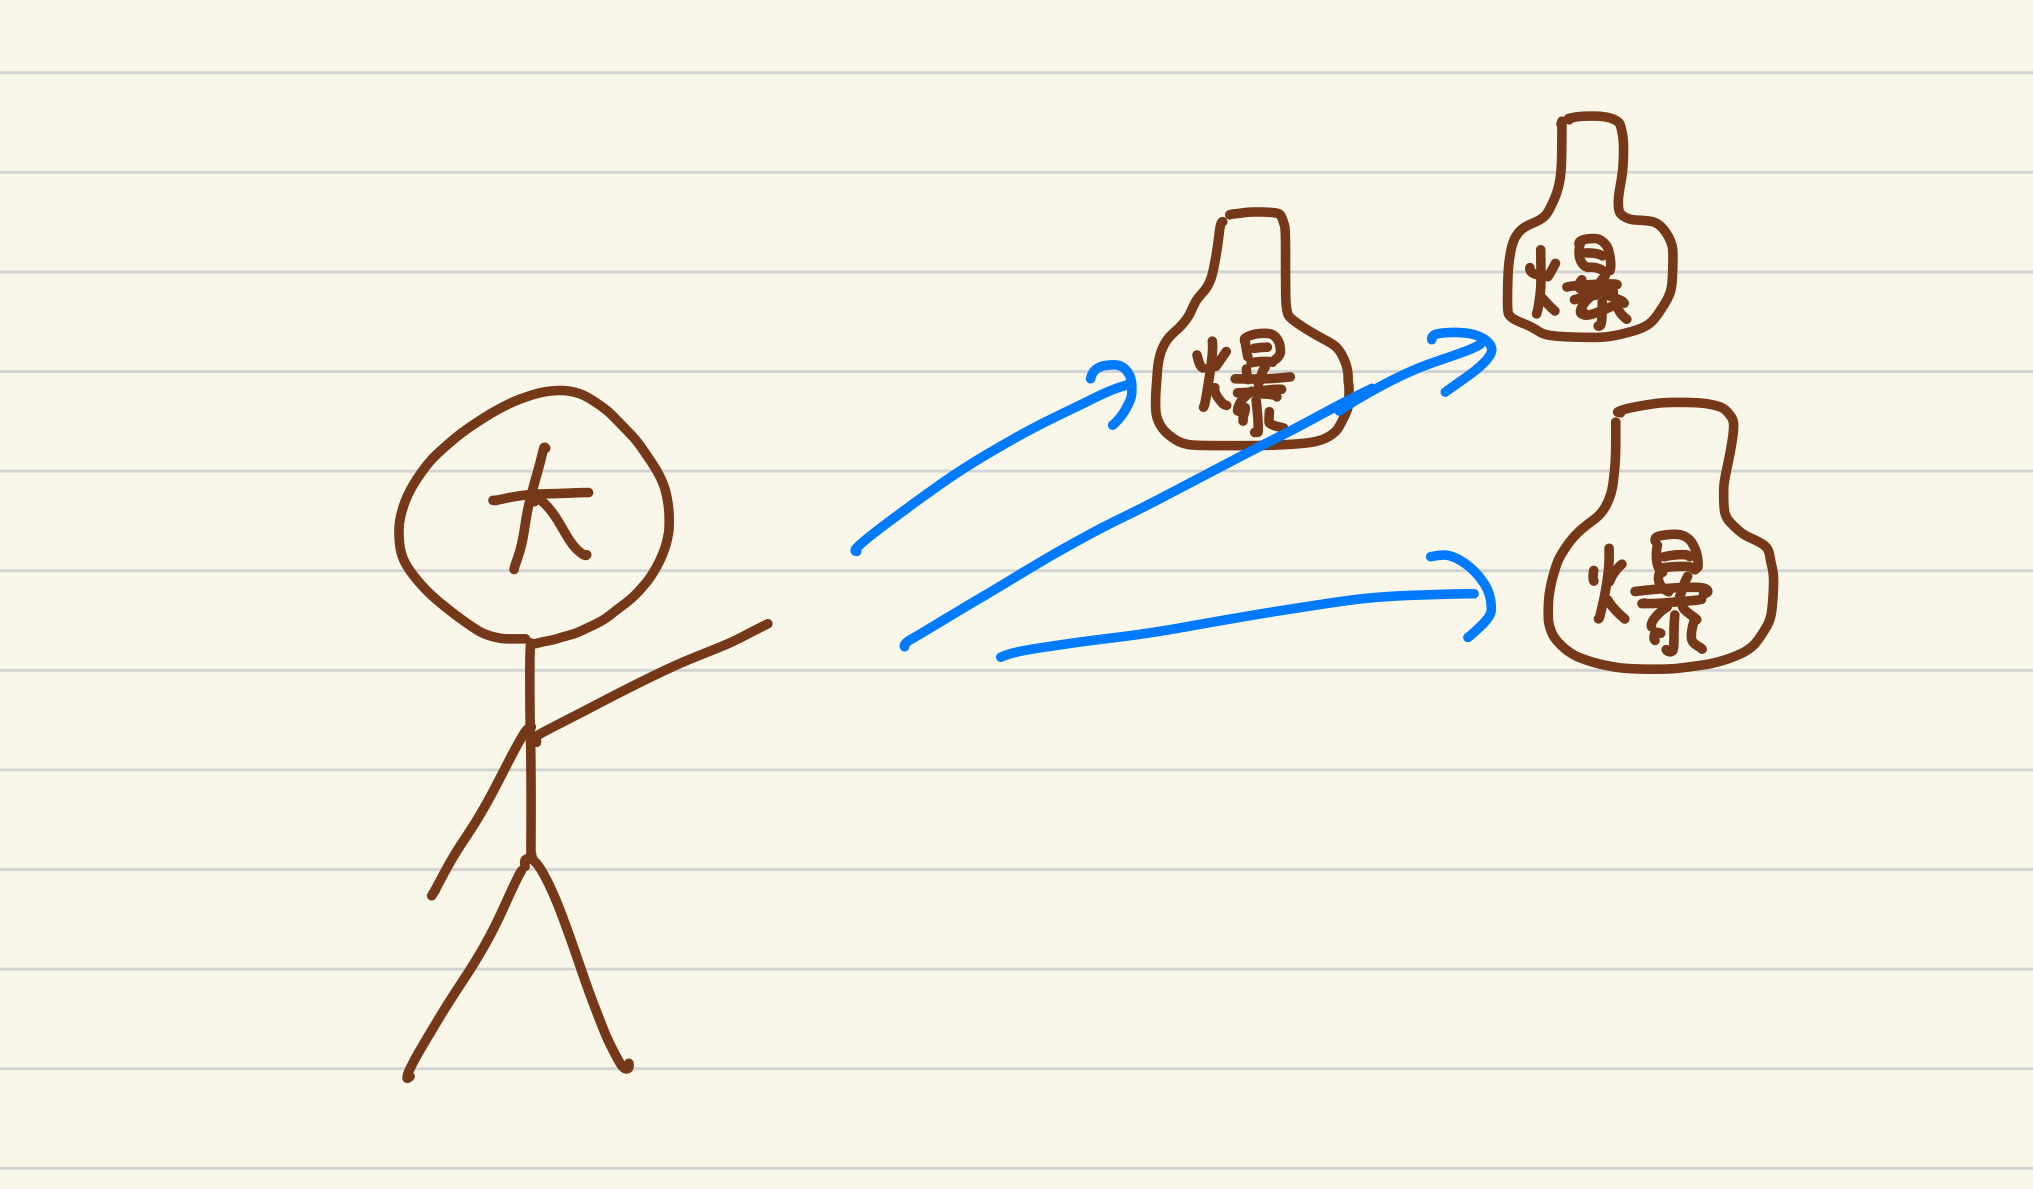
\includegraphics[width=12cm]{imags/tripleBakudan.eps}
    \caption{マルチエナドリ爆弾を投げる大学生}
  \end{center}
\end{figure}

\newpage

・マルチエナドリの仕様
\begin{enumerate}
  \item 左右に投げられる
  \item エナドリ爆弾を3個投げる
  \item 投げる軌道は、少しずらす
  一個はエナドリ爆弾と同じ、一個はちょっと高め、一個はちょっと低め
  \begin{figure}[htbp]
    \begin{center}
      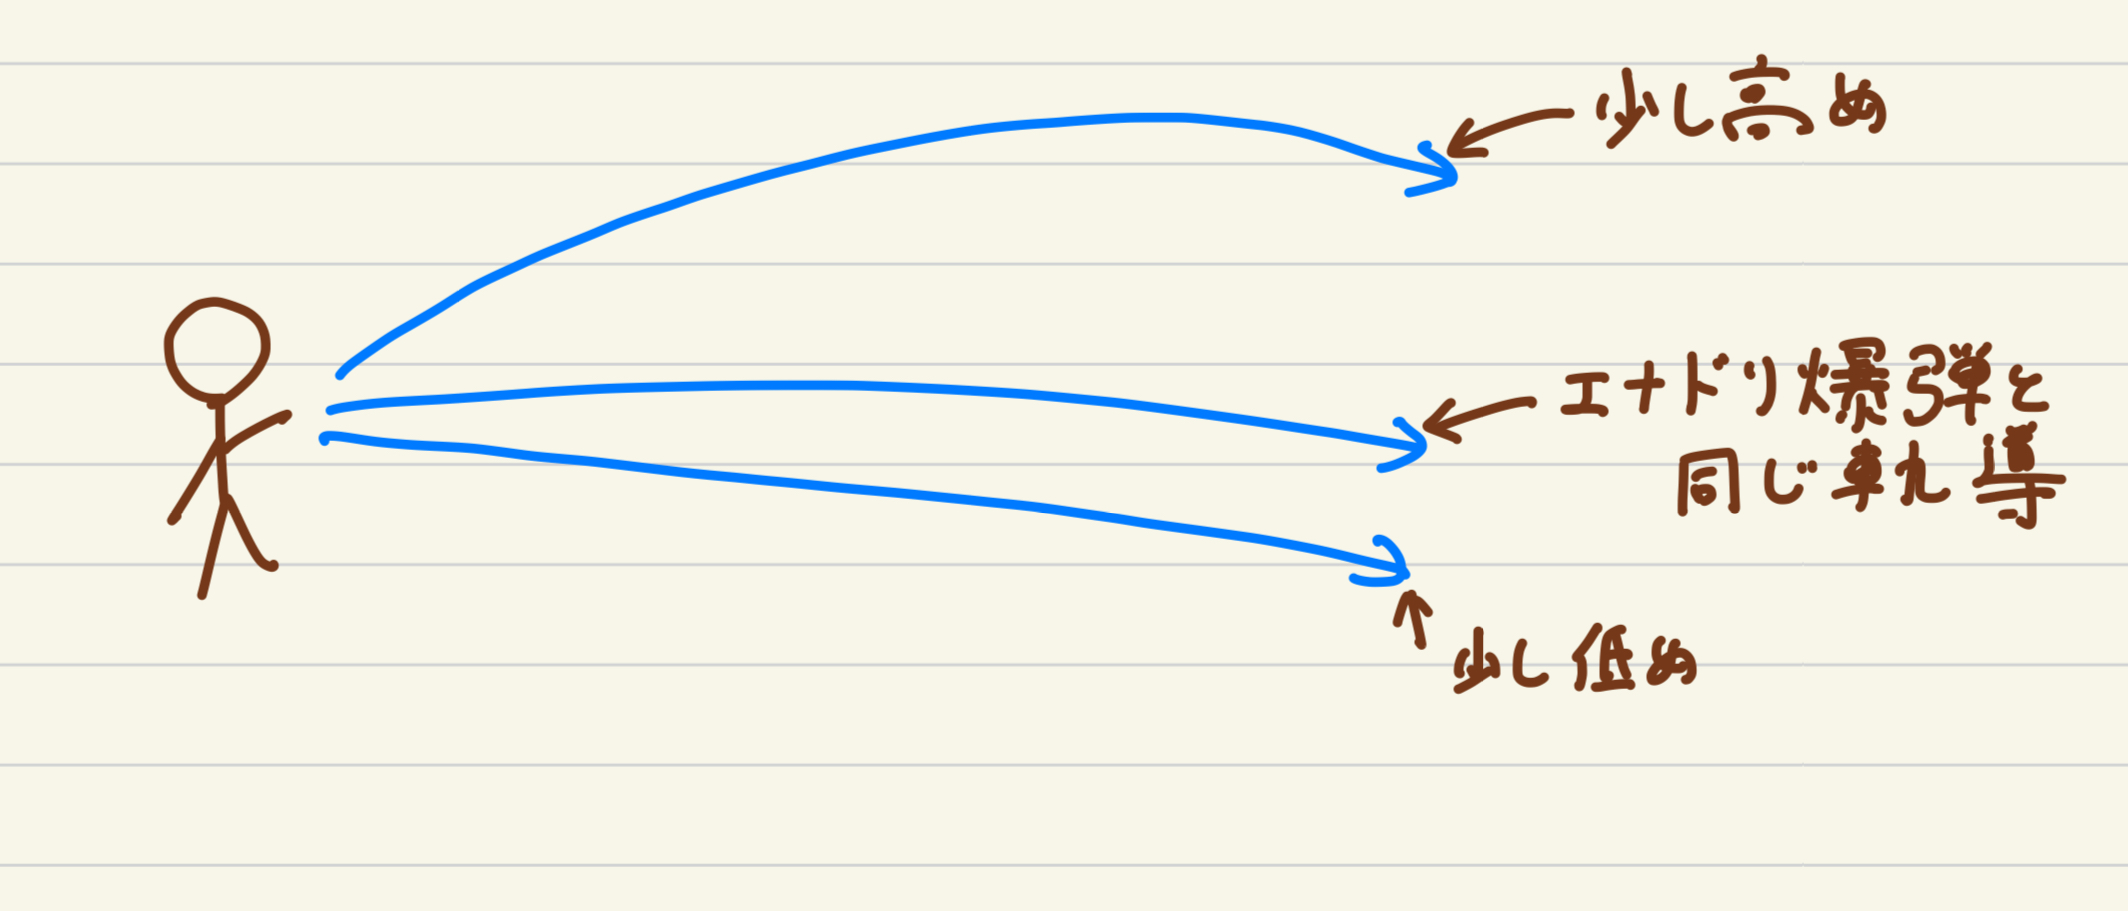
\includegraphics[width=12cm]{imags/tripleKidou.eps}
      \caption{マルチエナドリの軌道}
    \end{center}
  \end{figure}
  \item マルチエナドリを投げられる間、移動速度が80\% (要調整) になる
\end{enumerate}

\newpage

・箱エナドリ

エナドリボタンを2.6〜3.6秒押すと、箱エナドリを投げる。

箱エナドリは、何かに当たると弾けて、小エナドリ爆弾を大量にばら撒く。

小エナドリ爆弾は、それぞれ爆発する

\begin{figure}[htbp]
  \begin{center}
    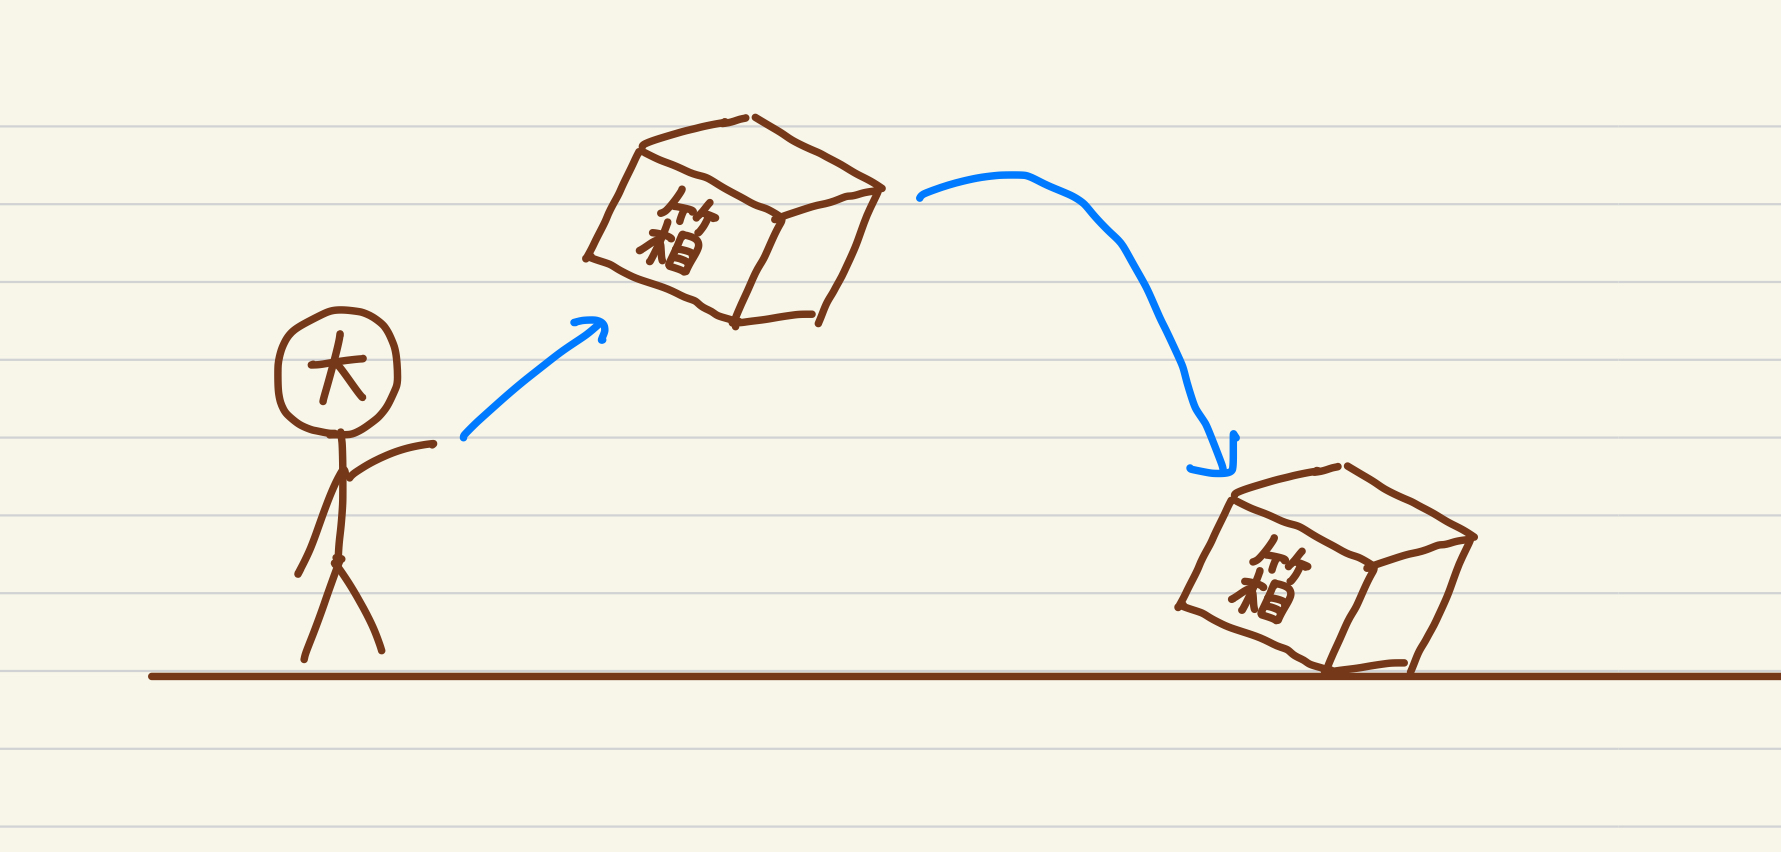
\includegraphics[width=12cm]{imags/hakoEnadori.eps}
    \caption{箱エナドリを投げる大学生}
  \end{center}
\end{figure}

\begin{figure}[htbp]
  \begin{center}
    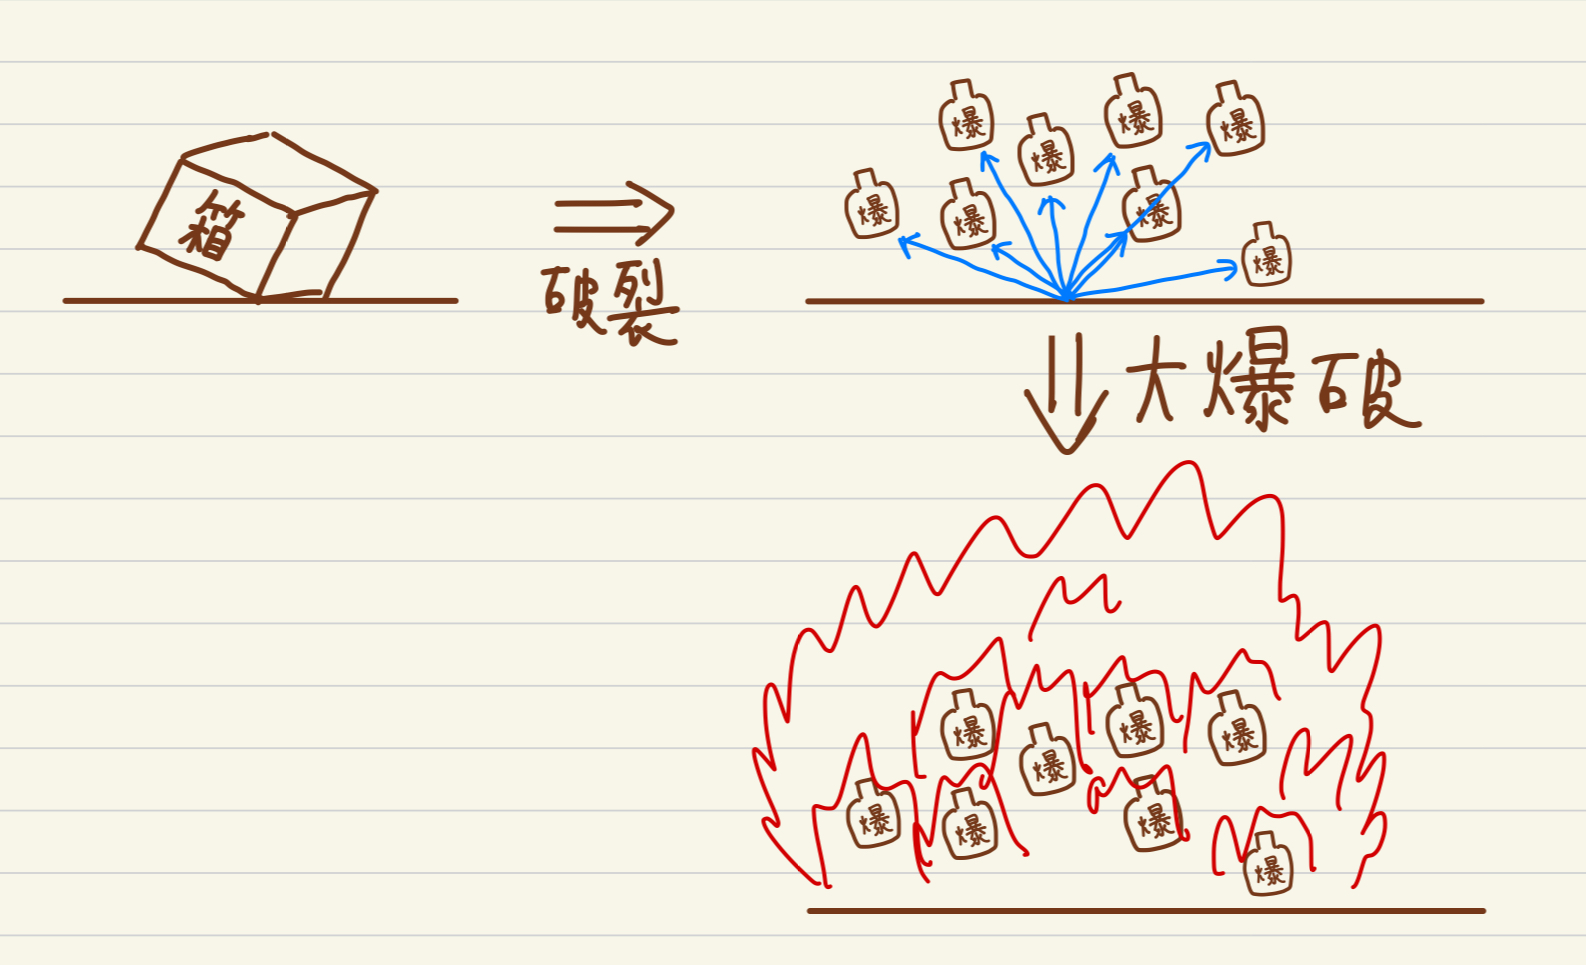
\includegraphics[width=12cm]{imags/hakoEnadoriBakuha.eps}
    \caption{箱エナドリの爆発の手順}
  \end{center}
\end{figure}

\newpage




\end{document}
